\documentclass[10pt,xcolor={svgnames}]{beamer}
%\usefonttheme[onlymath]{serif}
%%%%% Colors
\usetheme{Dresden}%\usetheme{Madrid}
\colorlet{beamer@blendedblue}{green!55!black}
%%%%%

%%%%% Other 
\beamertemplatenavigationsymbolsempty
\addtobeamertemplate{navigation symbols}{}{%
    \usebeamerfont{footline}%
    \usebeamercolor[fg]{footline}%
    \hspace{1em}%
    \insertframenumber/\inserttotalframenumber
}
\usepackage{hyperref, url}
%\usepackage[symbol]{footmisc}

\definecolor{pine_green}{HTML}{007935}
\hypersetup{colorlinks,breaklinks,linkcolor=white,urlcolor=orange,citecolor=black}
\renewcommand\thefootnote{\textcolor{pine_green}{\arabic{footnote}}}
\setbeamercolor{alerted text}{fg=pine_green}

\renewcommand{\i}{\mathnormal{I}}

\usepackage{cancel}
\usepackage{ulem}
\usepackage{multirow}
\usepackage{mathtools}
\usepackage{makecell}
\DeclarePairedDelimiter{\abs}{\lvert}{\rvert}
\renewcommand{\epsilon}{\varepsilon}
\setbeamertemplate{itemize subitem}{\textbullet}
\setbeamertemplate{itemize subsubitem}{$\circ$}

%https://tex.stackexchange.com/questions/289542/auto-resizing-parenthesis-in-math-formulas
% \usepackage{amsmath} for testing
\newcommand*\autoop{\left(}
\newcommand*\autocp{\right)}
\newcommand*\autoob{\left[}
\newcommand*\autocb{\right]}
\AtBeginDocument {%
   \mathcode`( 32768
   \mathcode`) 32768
   \mathcode`[ 32768
   \mathcode`] 32768
   \begingroup
       \lccode`\~`(
       \lowercase{%
   \endgroup
       \let~\autoop
   }\begingroup
       \lccode`\~`)
       \lowercase{%
   \endgroup
       \let~\autocp
   }\begingroup
       \lccode`\~`[
       \lowercase{%
   \endgroup
       \let~\autoob
   }\begingroup
       \lccode`\~`]
       \lowercase{%
   \endgroup
       \let~\autocb
   }}

\delimiterfactor 1001

\makeatletter
% for amsmath "compatibility" (not sophisticated)
% \usepackage{amsmath}
\AtBeginDocument {%
          \def\resetMathstrut@{%
           \setbox\z@\hbox{\the\textfont\symoperators\char40}%
           \ht\Mathstrutbox@\ht\z@ \dp\Mathstrutbox@\dp\z@}%
}%
\makeatother
%%%%%

%%%%% Greying out/invisible Slides
%\setbeamercovered{invisible}
%\setbeamercovered{%
%  again covered={\opaqueness<1->{15}}}
  
%%%%%







%%%%% Footnotes and captions
%\usepackage[utf8]{inputenc}
\usepackage{caption}
\usepackage{comment}
\setbeamerfont{footnote}{size=\tiny}
\setbeamerfont{caption}{size=\small}
%\setbeamerfont{normal text}{size=\small}
\setbeamerfont{itemize/enumerate body}{size=\small}
\setbeamerfont{itemize/enumerate subbody}{size=\footnotesize}
%%%%%


%%%%
\usepackage{booktabs}
\usepackage{multirow,bigstrut}
\usepackage{tabu}

%%%%



%Information to be included in the title page:
\title[Connor Wiegand]{Intro to Economic Analysis: Microeconomics}
\subtitle{EC 201 - Day 13 Slides}
\author[EC 201]{Connor Wiegand}
\institute[]{Department of Economics - University of Oregon}
\date{8 November 2021}


\begin{document}

\frame{\titlepage}

\section*{Finish Up Basic Taxes/Subsides}

\begin{frame}{Logistics}
    \begin{itemize}
        \item Homework 5 due this Saturday at 11:59pm
        \item Next news assignments posted, due this Wednesday, Nov 10, at 11:59pm
        \item Midterm grades with grade update to come
    \end{itemize}
\end{frame}

\begin{frame}{Recall -- Tax Motivation}
    \begin{itemize}
        \item There are many ways to talk about taxes/subsidies, we will solely focus on per-unit taxes in this class
        \item We may tax (subsidize, resp.) consumers to discourage (encourage) consumption, and we may tax (subsidize) producers to discourage (encourage) production
        \item For a demand curve $P=mQ+b$, a tax $t$ shifts demand down by $t$ units, to $P=mQ+b-t$
        \item Conversely, a subsidy $s$ shifts demand up by $s$ units, to $P=mQ+b+s$
    \end{itemize}
\end{frame}

\begin{frame}{Recall -- Tax Effects}
    \begin{itemize}
        \item For a supply curve $P=mQ+b$, a tax $t$ shifts supply \underline{up} by $t$ units, to $P=mQ+b+t$
        \item Conversely, a subsidy $s$ shifts supply \underline{down} by $s$ units, to $P=mQ+b-s$
        \begin{itemize}
            \item This is because a tax on \textit{consumers} induces the price paid, $P$, to be replaced with $P+t$ \item While a tax on \textit{producers} induces the price received, $P$, to be replaced with $P-t$
        \end{itemize}
        \item Taxes and subsidies induce \textit{two} different notions of price in our market: prices paid by consumers, and prices received by producers
        \item It's still the case that taxes have a negative, regressive effect on supply/demand, while subsidies have a positive, stimulative effect on supply/demand
        \begin{itemize}
            \item It just looks backward because of the difference in slopes for supply/demand
        \end{itemize}
    \end{itemize}
\end{frame}

\begin{frame}{Example -- A Tax on Producers}
    \begin{itemize}[<+->]
        \item Suppose we want to discourage the rate at which businesses frack oil, and we do so by putting a \$40/unit tax on production
        \item This is visualized as
        \begin{figure}
            \centering
            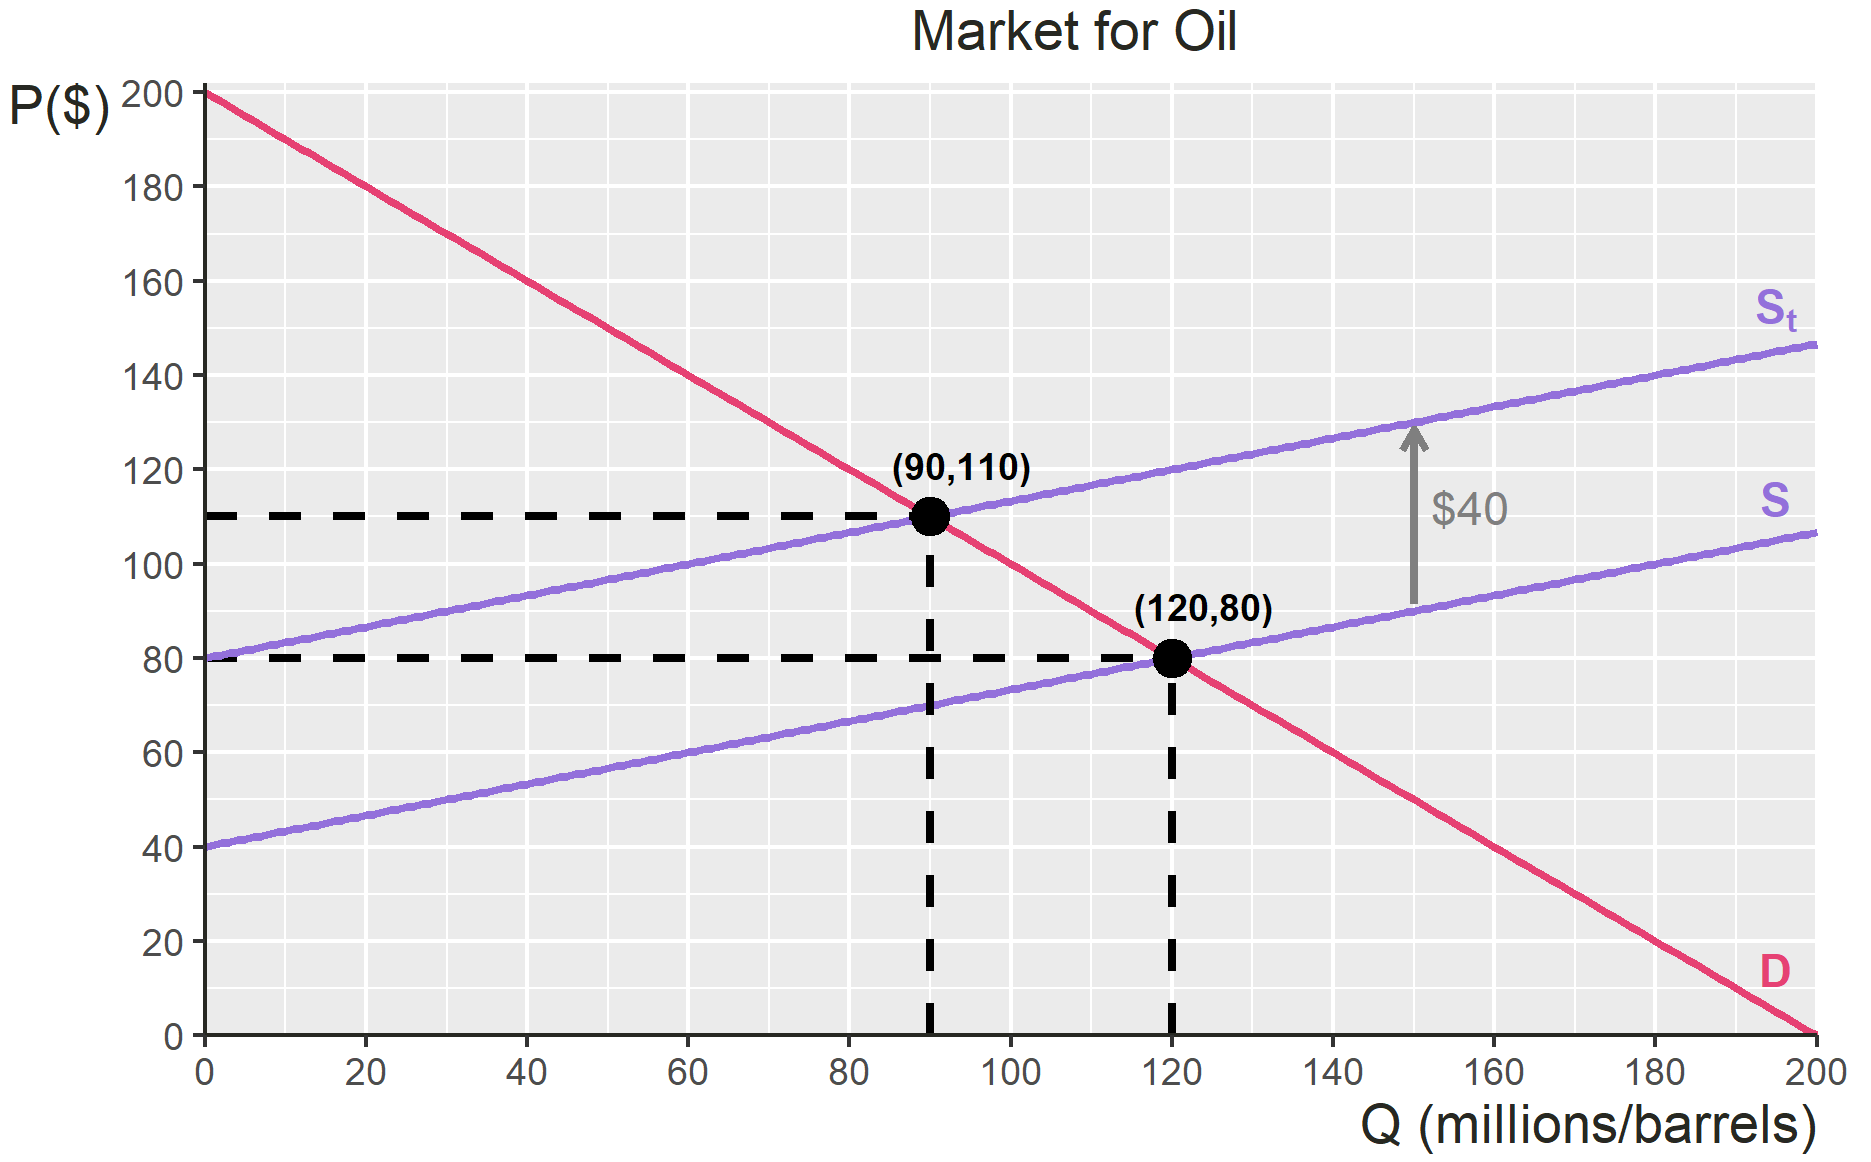
\includegraphics[width=8cm]{Oil tax.png}
            \caption*{The supply line shifts from $S$ to $S_{t}$ with the tax}
        \end{figure}
    \end{itemize}
\end{frame}

\begin{frame}{Difference in Prices -- Tax on Producers}
    \begin{itemize}[<+->]
        \item Now, the producer charges the consumer $\$110$/barrel for oil, but must give $\$40$ for each unit to the government
        \item This is visualized as
        \begin{figure}
            \centering
            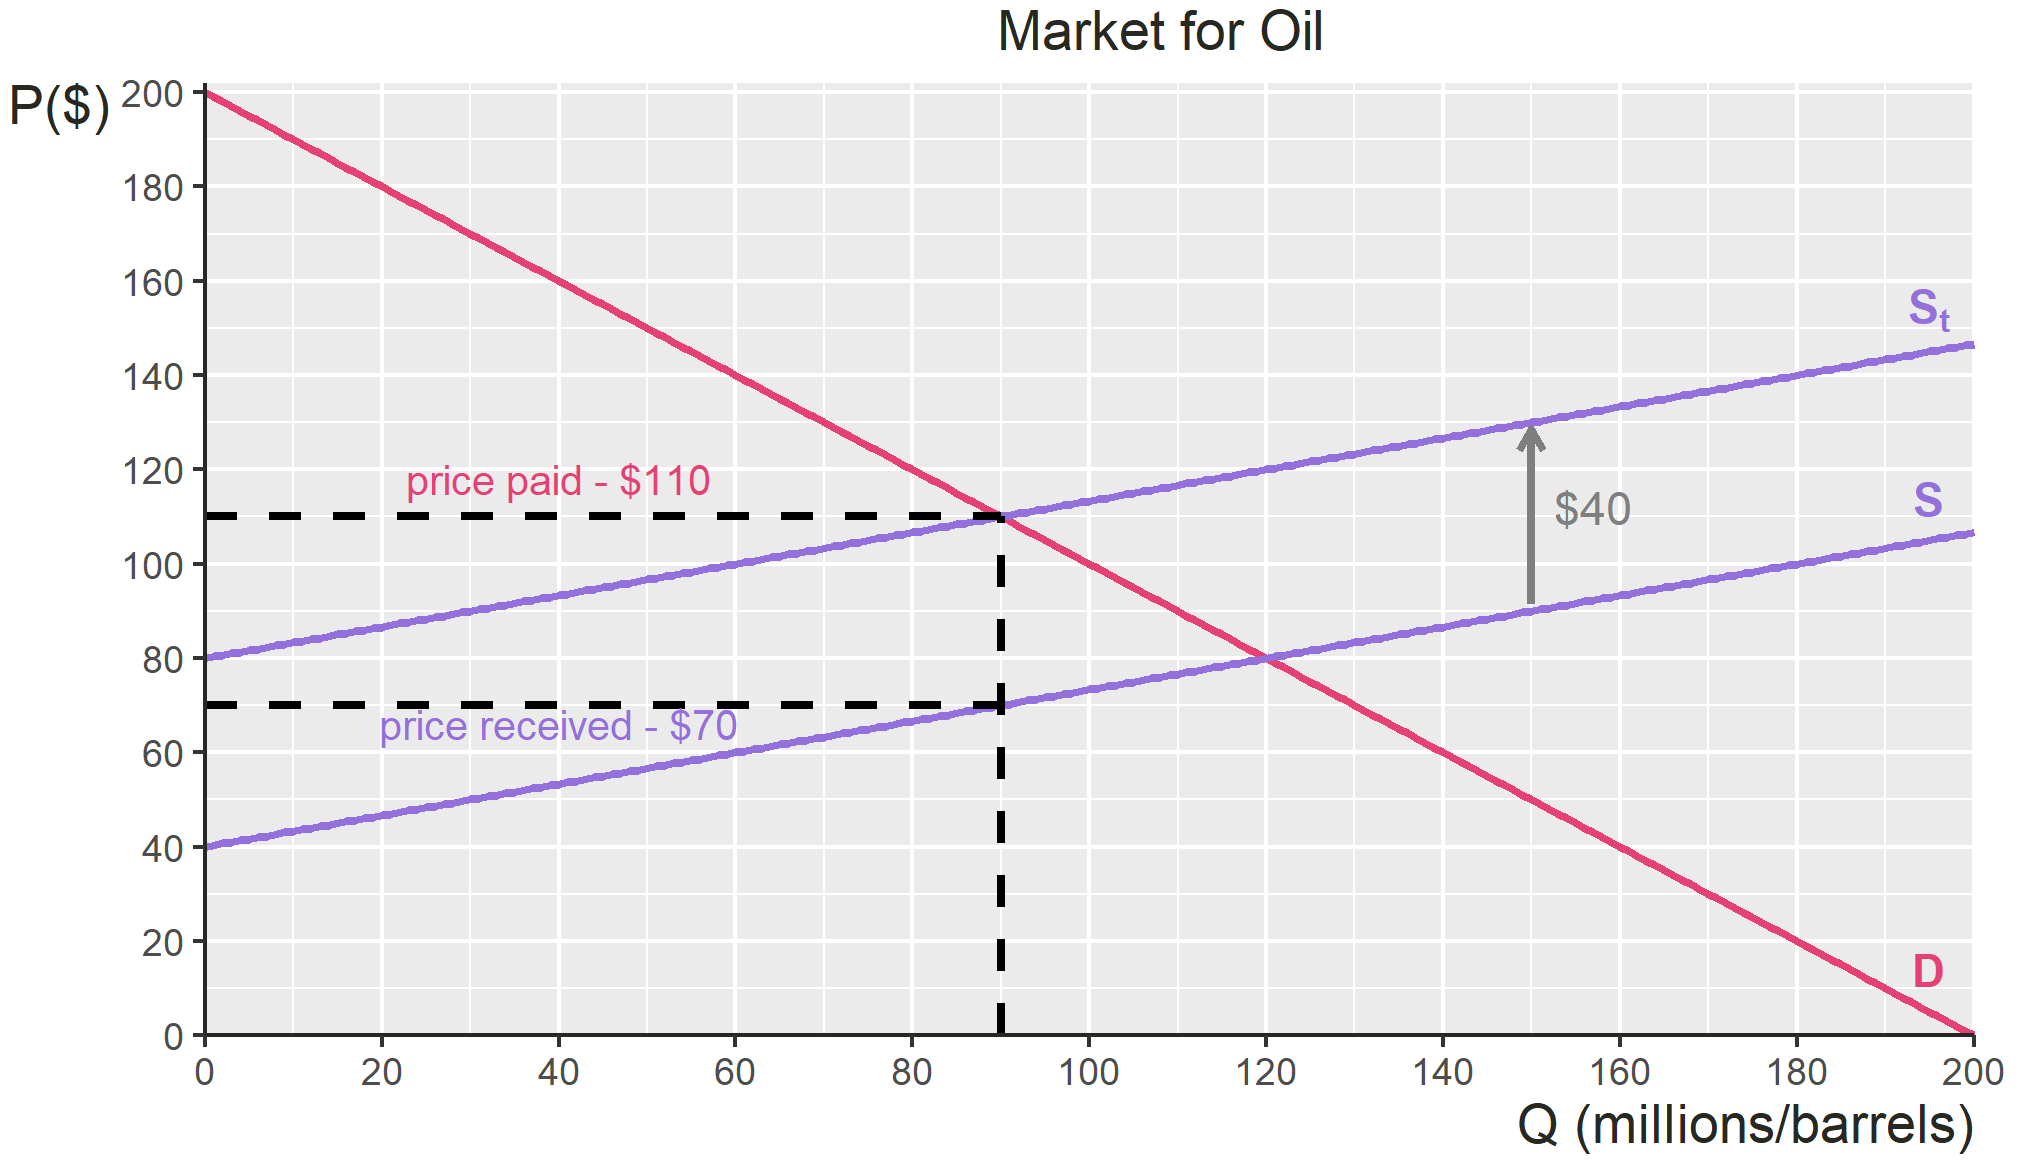
\includegraphics[width=8cm]{Oil tax prices.png}
        \end{figure}
    \end{itemize}
\end{frame}

\begin{frame}{Government Revenue -- Tax on Producers}
    \begin{itemize}[<+->]
        \item What is government revenue under this policy?
        \item At \$40/unit times 90 units, 
        $$GR=(40)(90M)=\$3.6B$$
        \begin{figure}
            \centering
            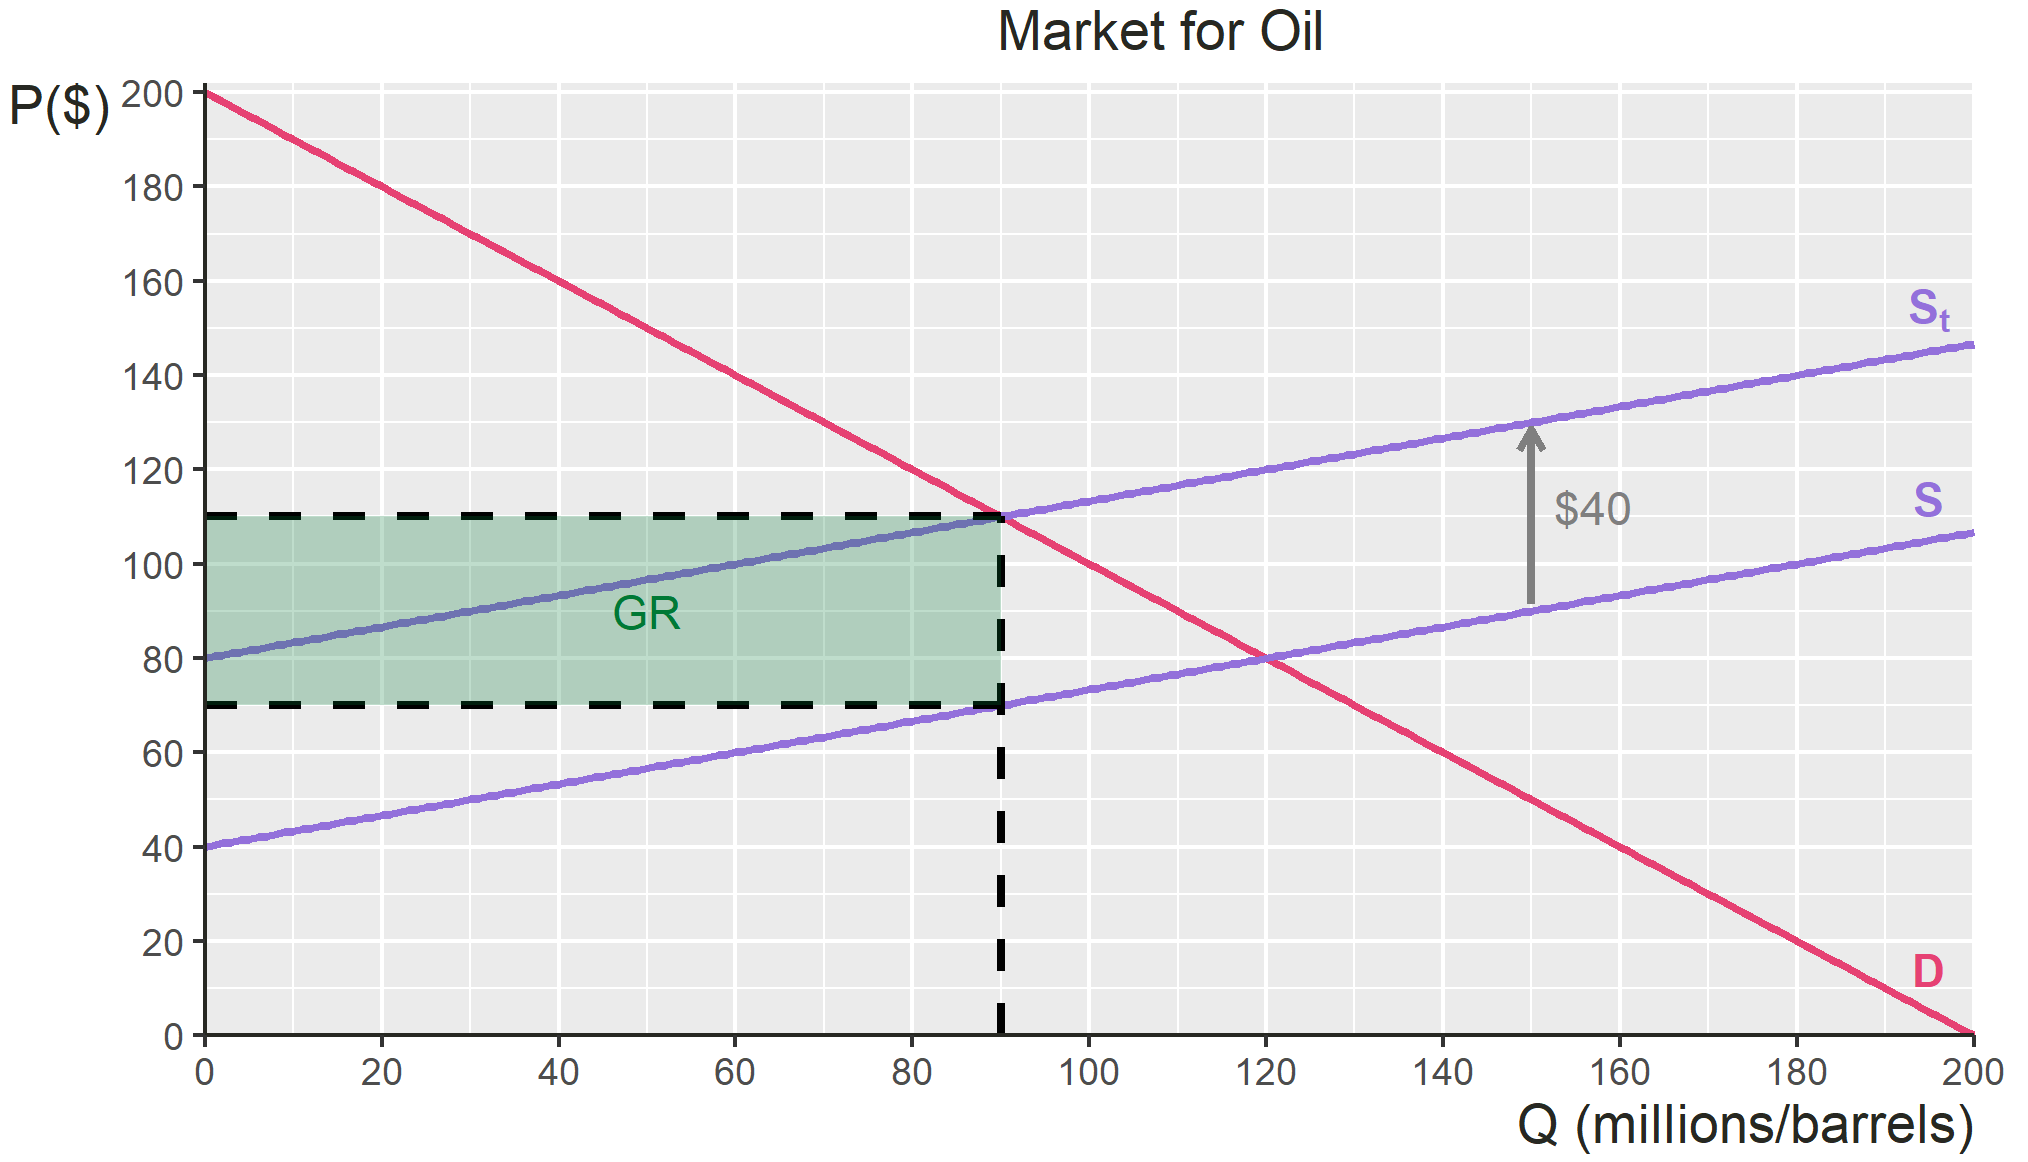
\includegraphics[width=8cm]{Oil tax gr.png}
            \caption*{If we weren't working in millions, it would be $\$3600$}
        \end{figure}
    \end{itemize}
\end{frame}

\begin{frame}{Example -- A Subsidy for Producers}
    \begin{itemize}[<+->]
        \item Suppose that, in order to encourage wind power prominence, the government provides a $\$600$/unit subsidy to producers
        \begin{figure}
            \centering
            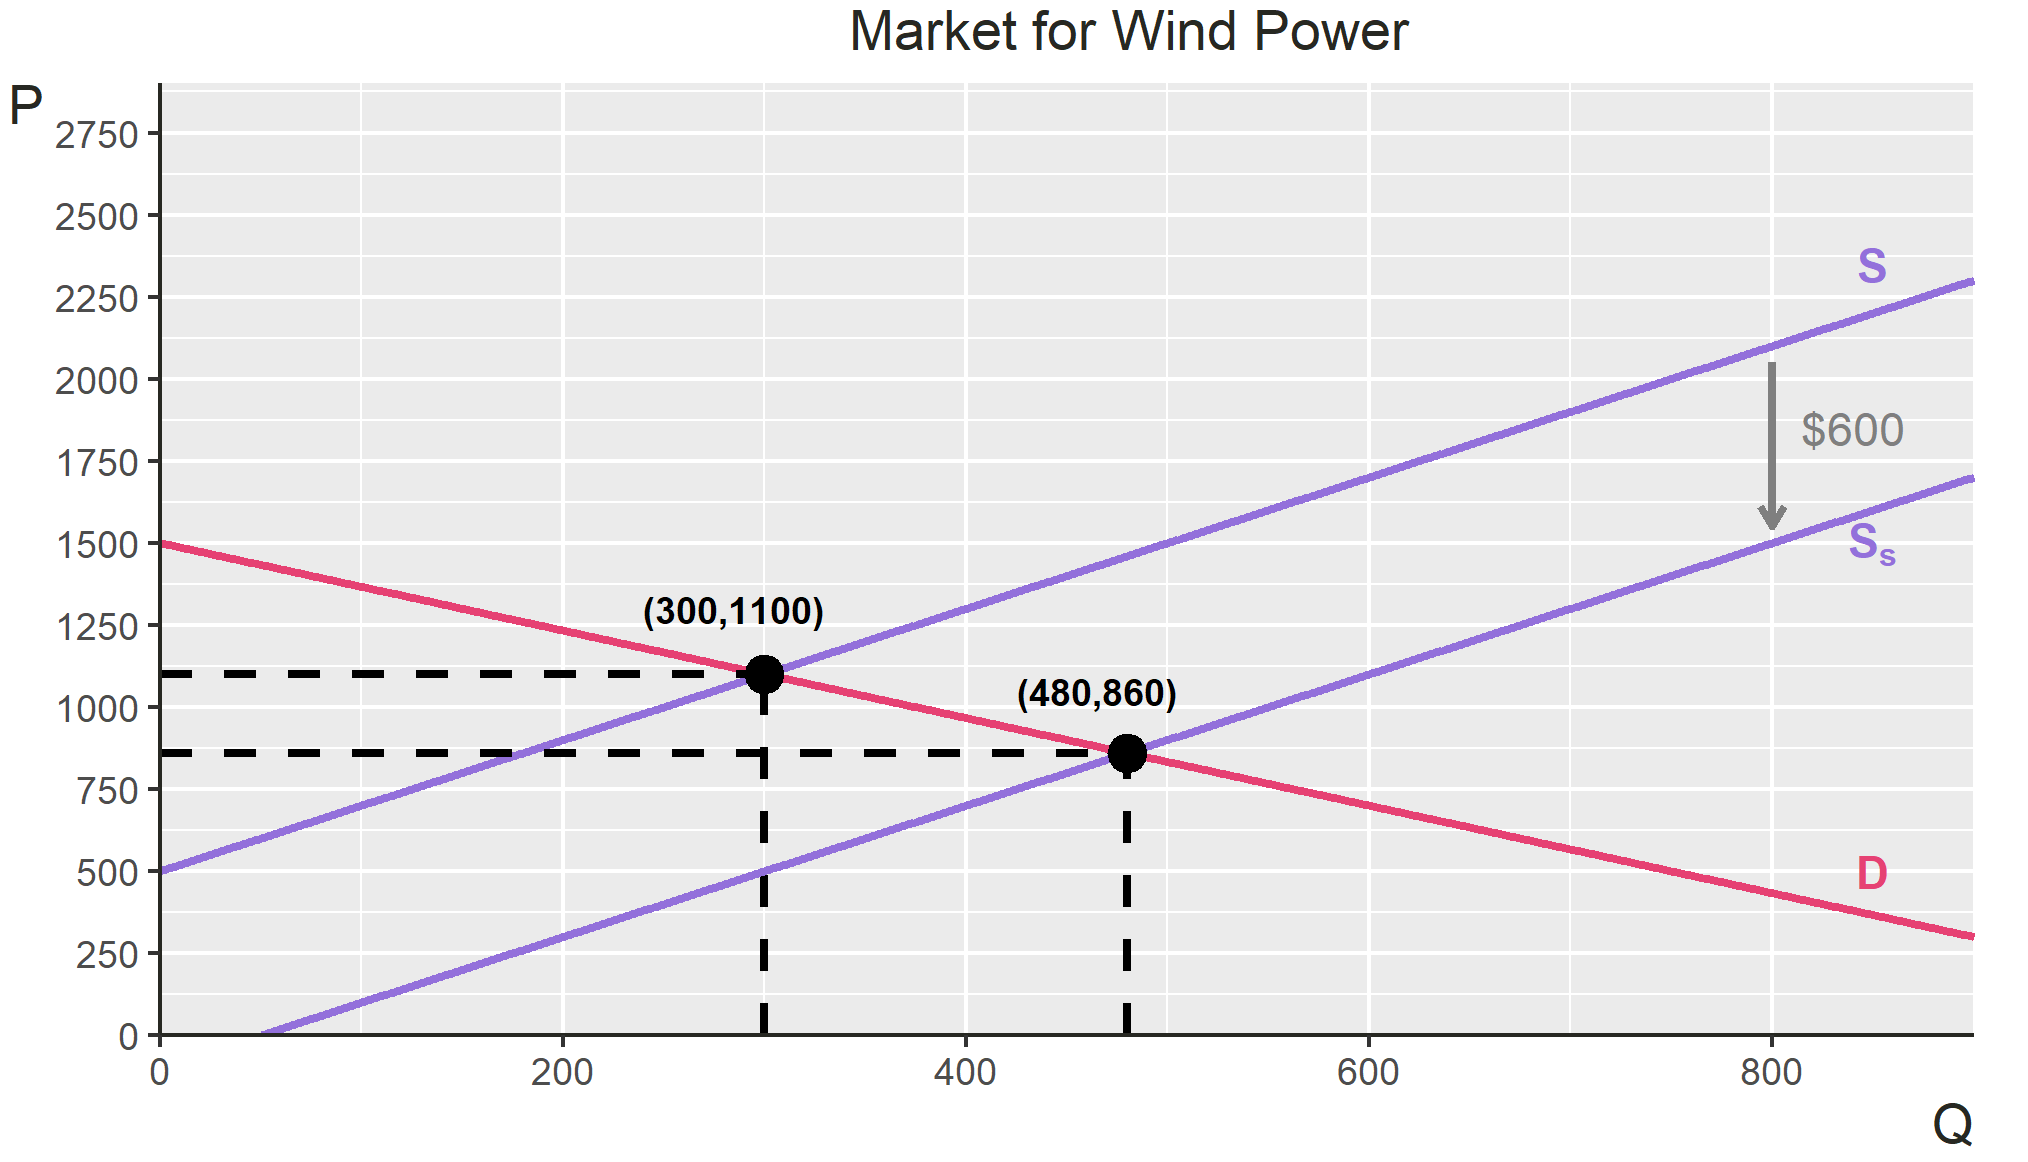
\includegraphics[width=8cm]{Wind sub.png}
            \caption*{The supply line shifts from $S$ to $S_{s}$ with the subsidy}
        \end{figure}
    \end{itemize}
\end{frame}

\begin{frame}{Difference in Prices -- Subsidy for Producers}
    \begin{itemize}[<+->]
        \item Now, the consumer pays $\$860$ for win power, and the producer gets $\$600$ extra for making and selling the wind power, meaning they receive $\$1460$
        \begin{figure}
            \centering
            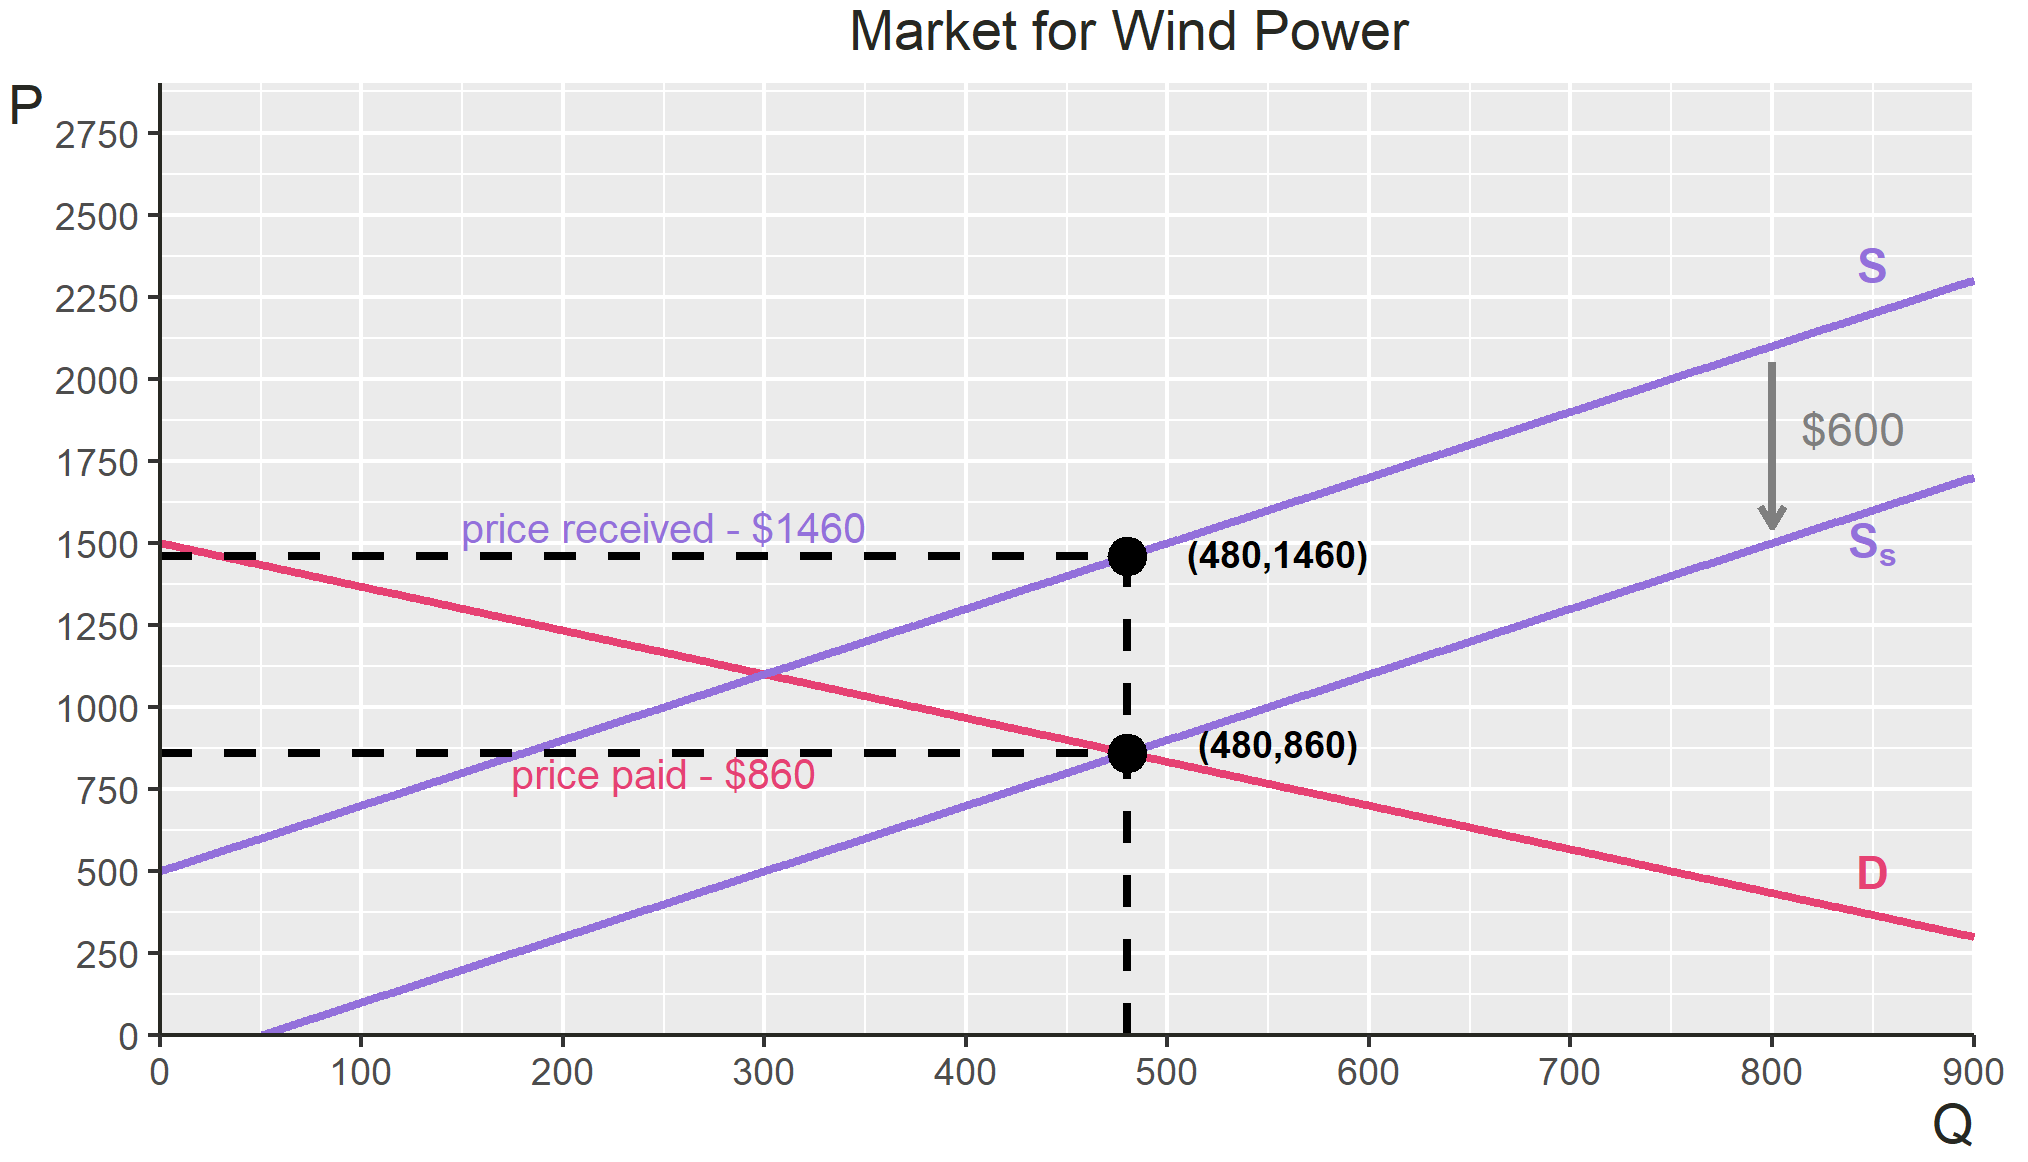
\includegraphics[width=8cm]{Wind sub prices.png}
        \end{figure}
    \end{itemize}
\end{frame}

\begin{frame}{Government Expenditure -- Subsidy for Producers}
    \begin{itemize}[<+->]
        \item What is government expenditure under this policy?
        \item At \$600/unit times 480 units, 
        $$GE=(600)(480)=\$288,000$$
        \item This is visualized as
        \begin{figure}
            \centering
            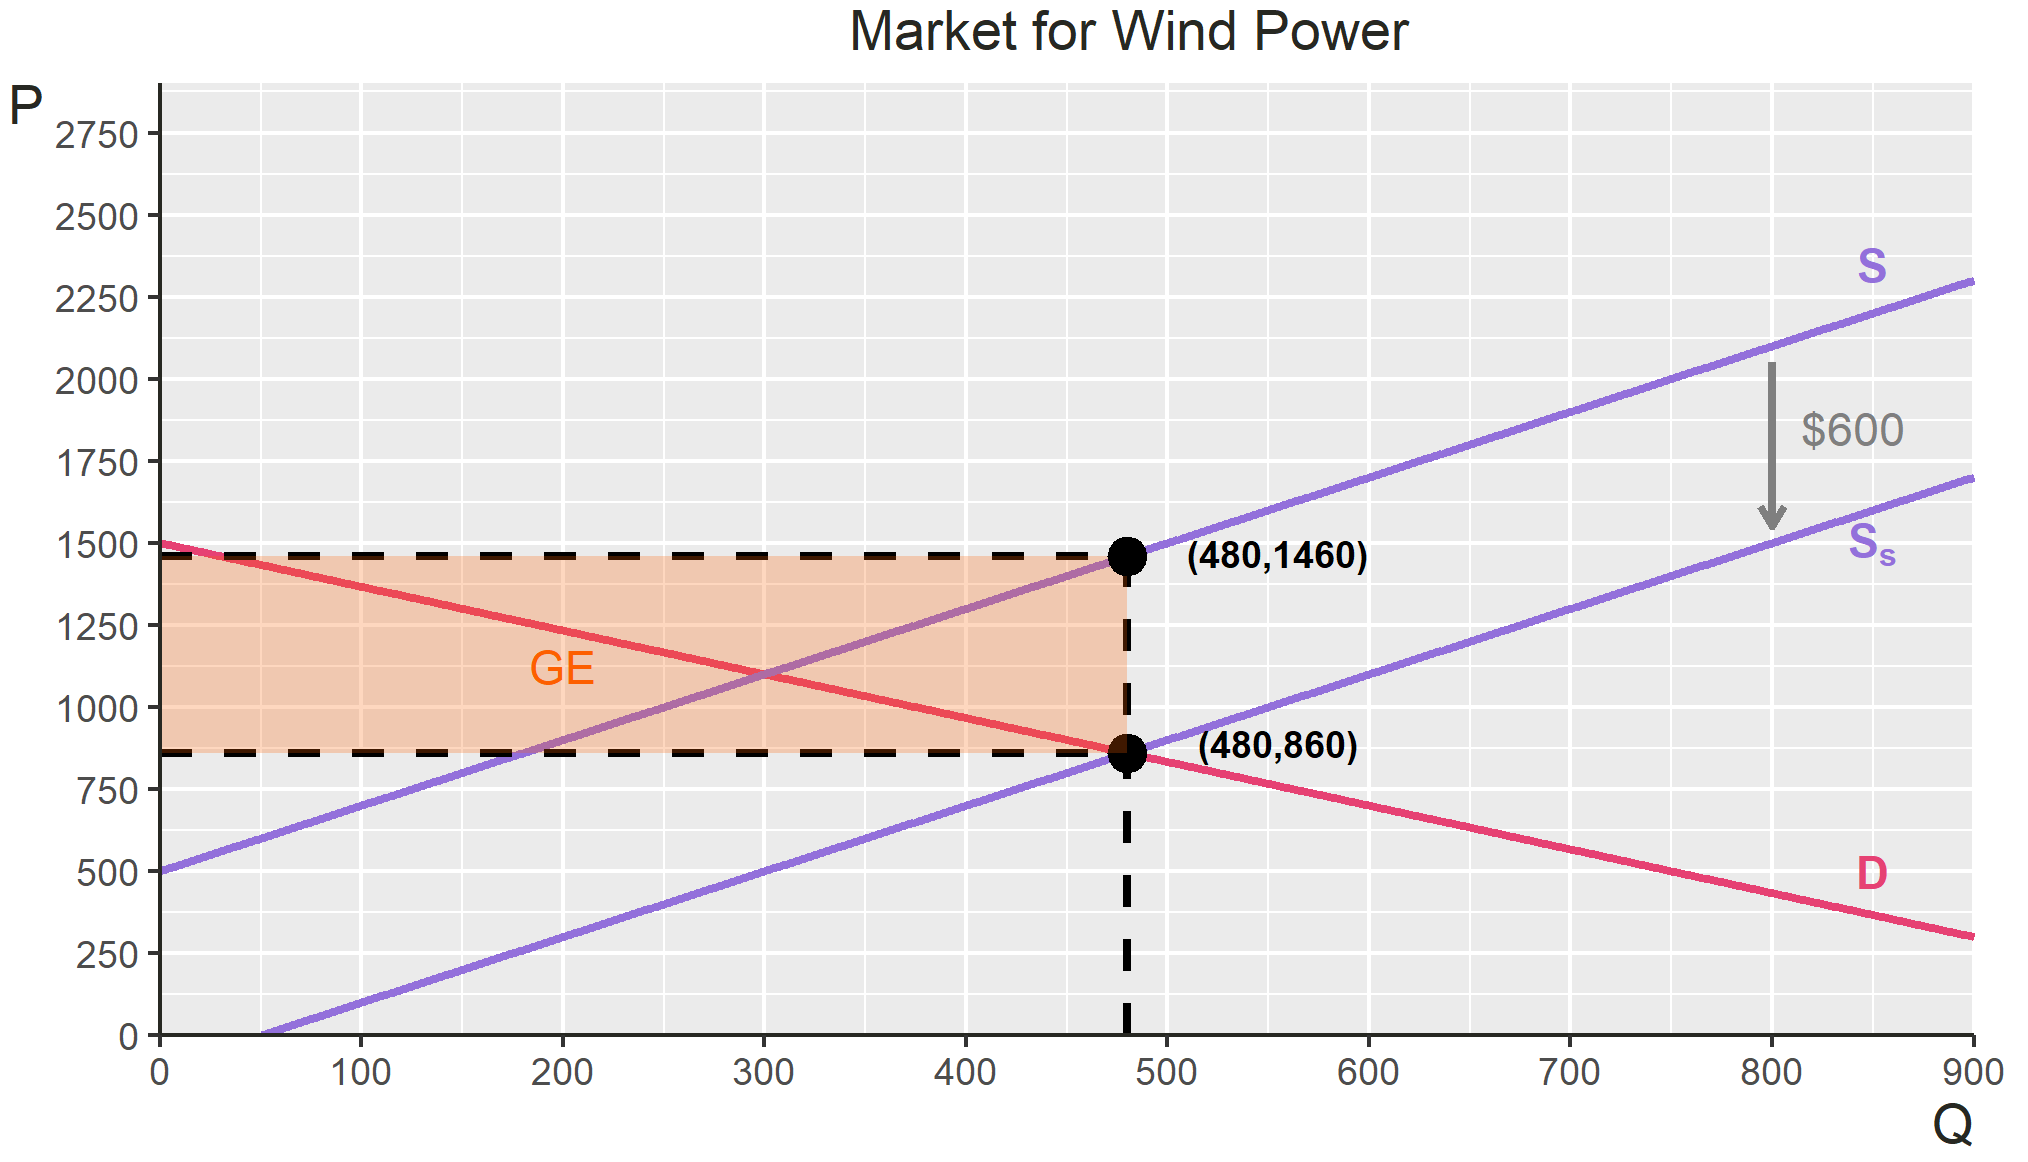
\includegraphics[width=8cm]{Wind sub ge.png}
        \end{figure}
    \end{itemize}
\end{frame}

\section*{Tax Burden}

\begin{frame}{Can Parties Just Pass on Taxes?}
    \begin{itemize}[<+->]
        \item You might be asking yourself: if we tax producers $\$4$ per unit of oil, wont, they just pass it on to consumers?
        \item Actually, no: one of the coolest things we can do, even at a basic level, is measure the relative tax burden that consumers and producers bear
        \item After thinking about it, especially under the lens of elasticity, this should make some sense:
        \begin{itemize}
            \item For example, when consumers are relatively elastic (compare to producers), they may not tolerate a large tax being passed down to them
            \item On the other hand, when producers are the elastic ones (compared to consumers), they can get away with passing most of a tax onto consumers
            \begin{itemize}
                \item This works the other way too, when the tax is on consumers: they may, effectively, ``pass" it to producers
            \end{itemize} 
        \end{itemize}
    \end{itemize}
\end{frame}

\begin{frame}{Defining the Tax Burden}
    \begin{itemize}[<+->]
        \item The tax burden is relatively simple to define
        \begin{itemize}
            \item For consumers, the tax burden is the difference between what consumers \textit{used to} pay, and what they \textit{currently} pay
            \item For producers, the tax burden is the difference between what producers \textit{used to} receive, and what they \textit{currently} receive
        \end{itemize}
        \item This is even easier to show graphically, let's look at some of our previous examples
    \end{itemize}
\end{frame}

\begin{frame}{Tax Burden -- Tax on Consumers}
    \begin{itemize}[<+->]
        \item Recall the $\$6$ tax on cigarettes, from our last class:
        \begin{figure}
            \centering
            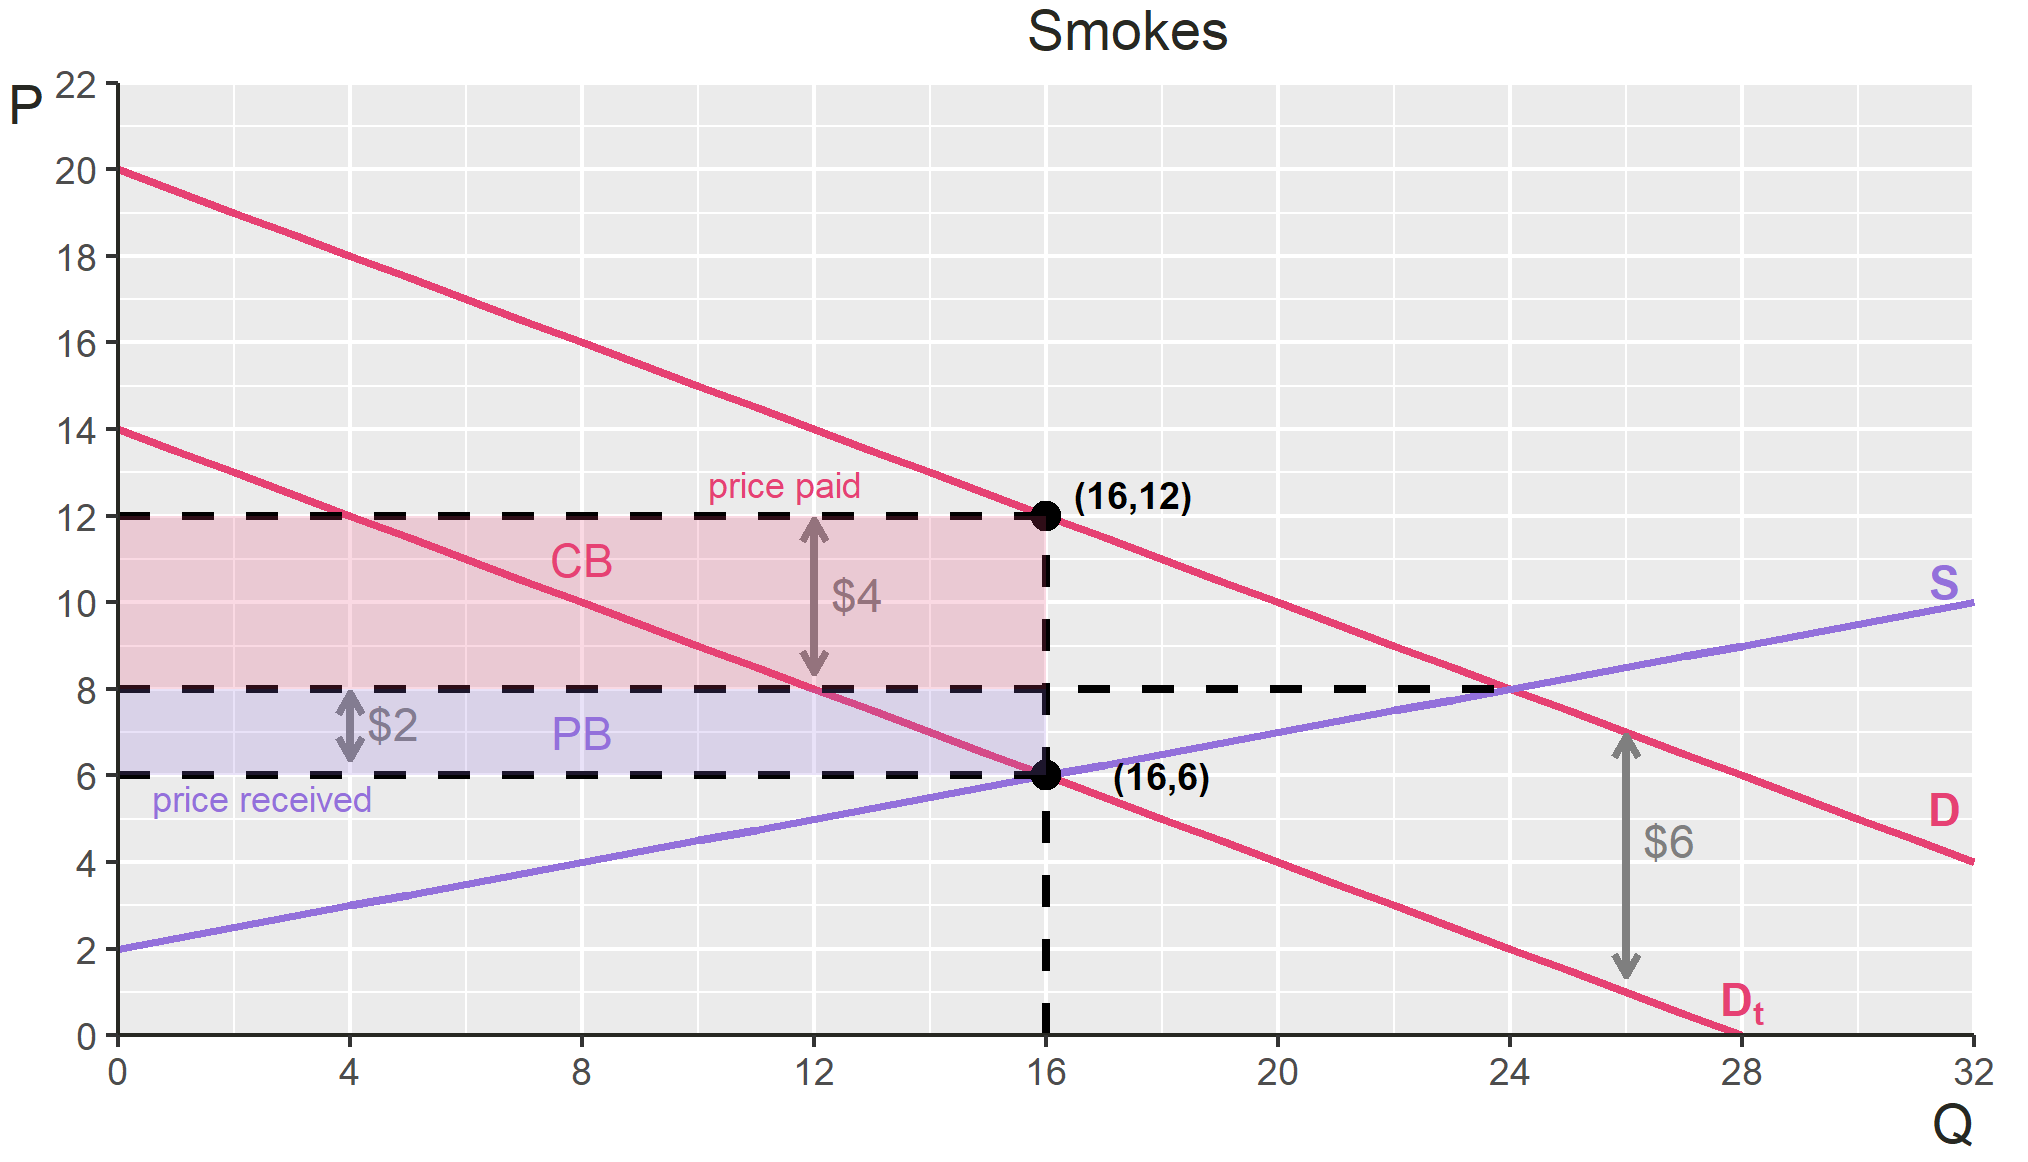
\includegraphics[width=7cm]{Dart tax gr.png}
        \end{figure}
        \item Consumers used to pay $\$8$ and producers used to receive $\$8$
        \item Now, consumers pay $\$12$/pack, and producers receive $\$6$/pack. Who is bearing what?
    \end{itemize}
\end{frame}

\begin{frame}{Tax Burden -- Tax on Consumers}
        \begin{figure}
            \centering
            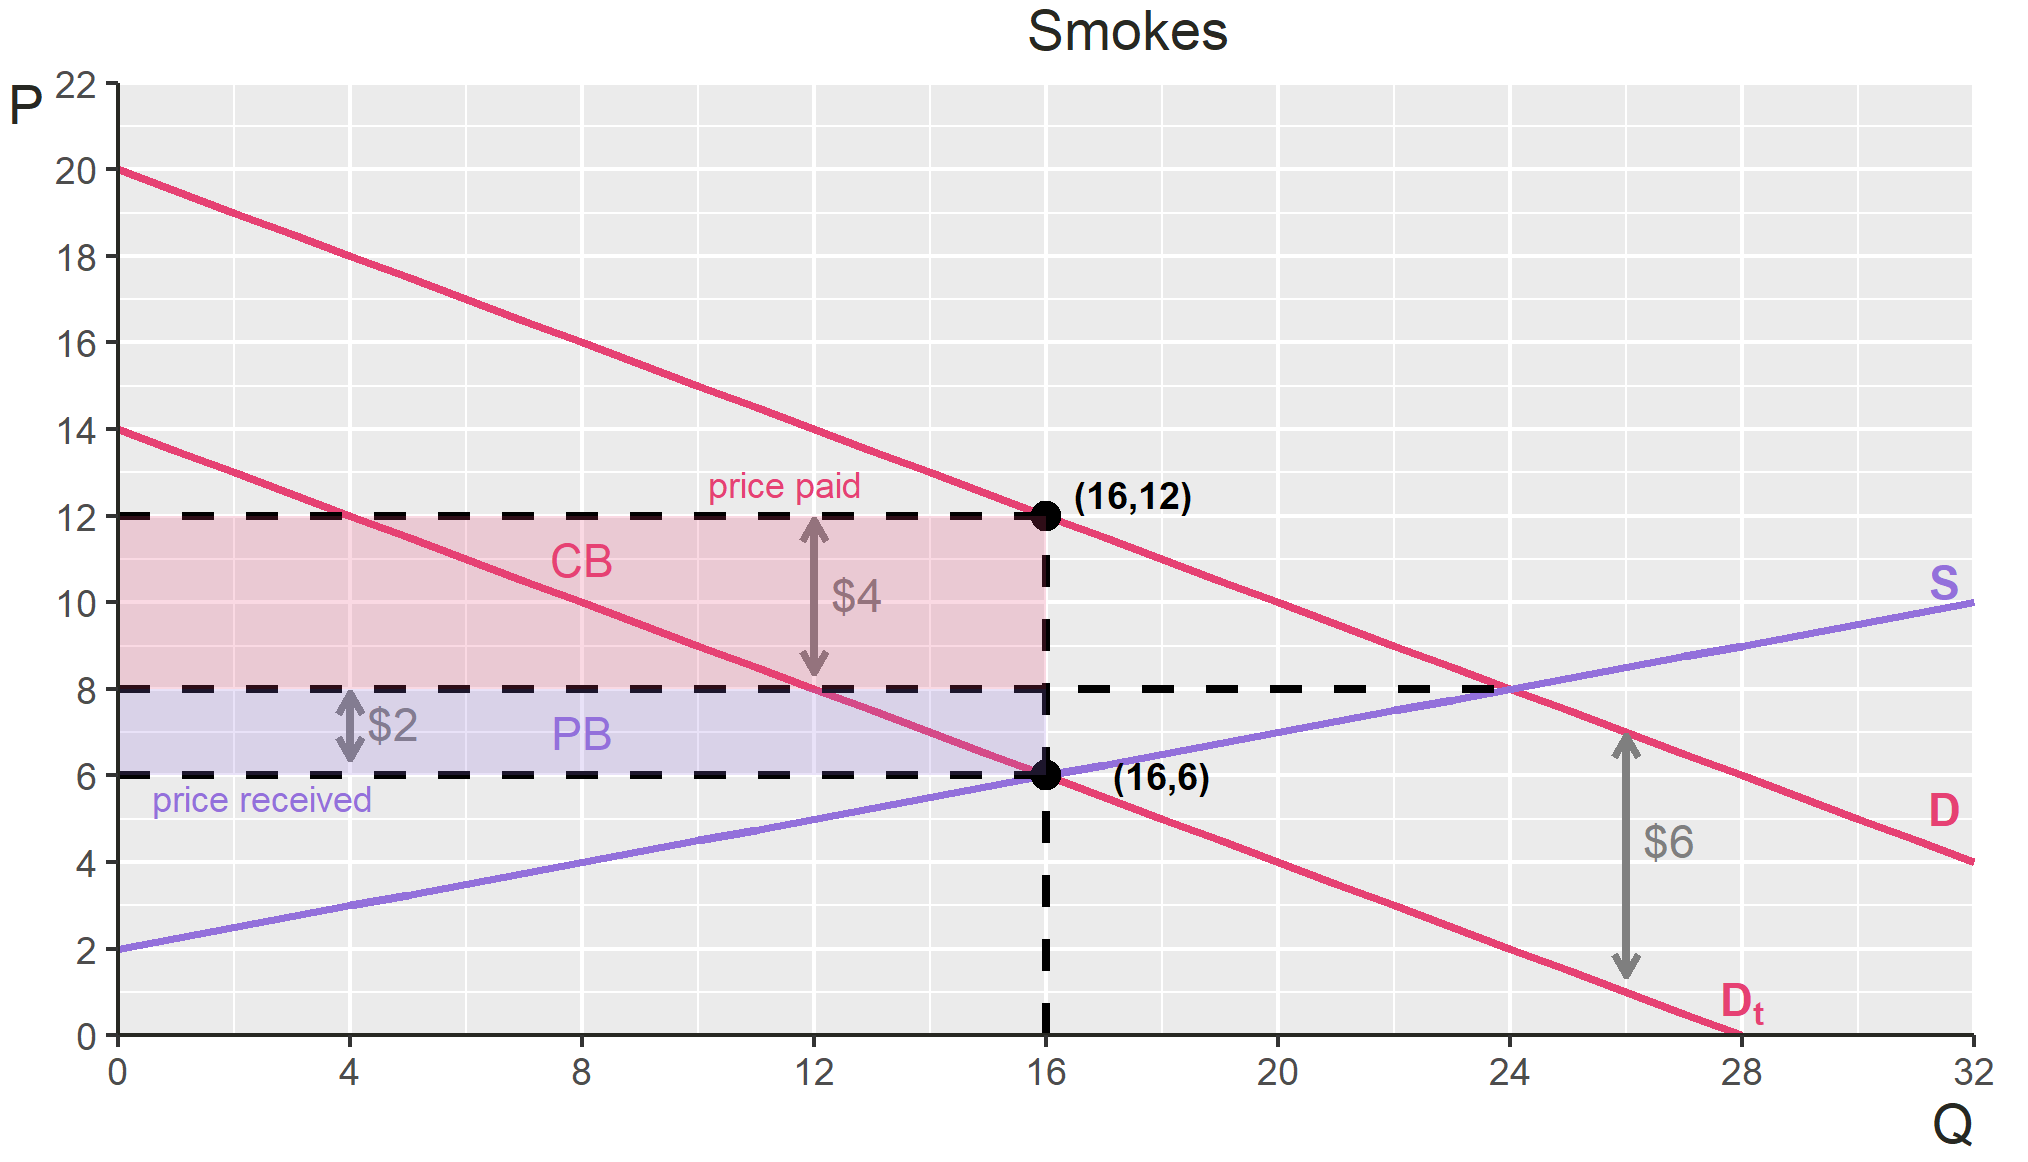
\includegraphics[width=8cm]{Dart tax burdens.png}
        \end{figure}
    \begin{itemize}[<+->]
    \vspace{-2mm}
        \item Consumers used to pay $\$8$, now they pay $\$12$: they pay $12-8=\$4$ of the burden, out of $\$6$
        \item Producers used to get $\$8$, now they get $\$6$: they pay $8-6=\$2$ of the burden, out of $\$6$
    \end{itemize}
\end{frame}

\begin{frame}{Tax Burden -- Tax on Consumers}
        \begin{figure}
            \centering
            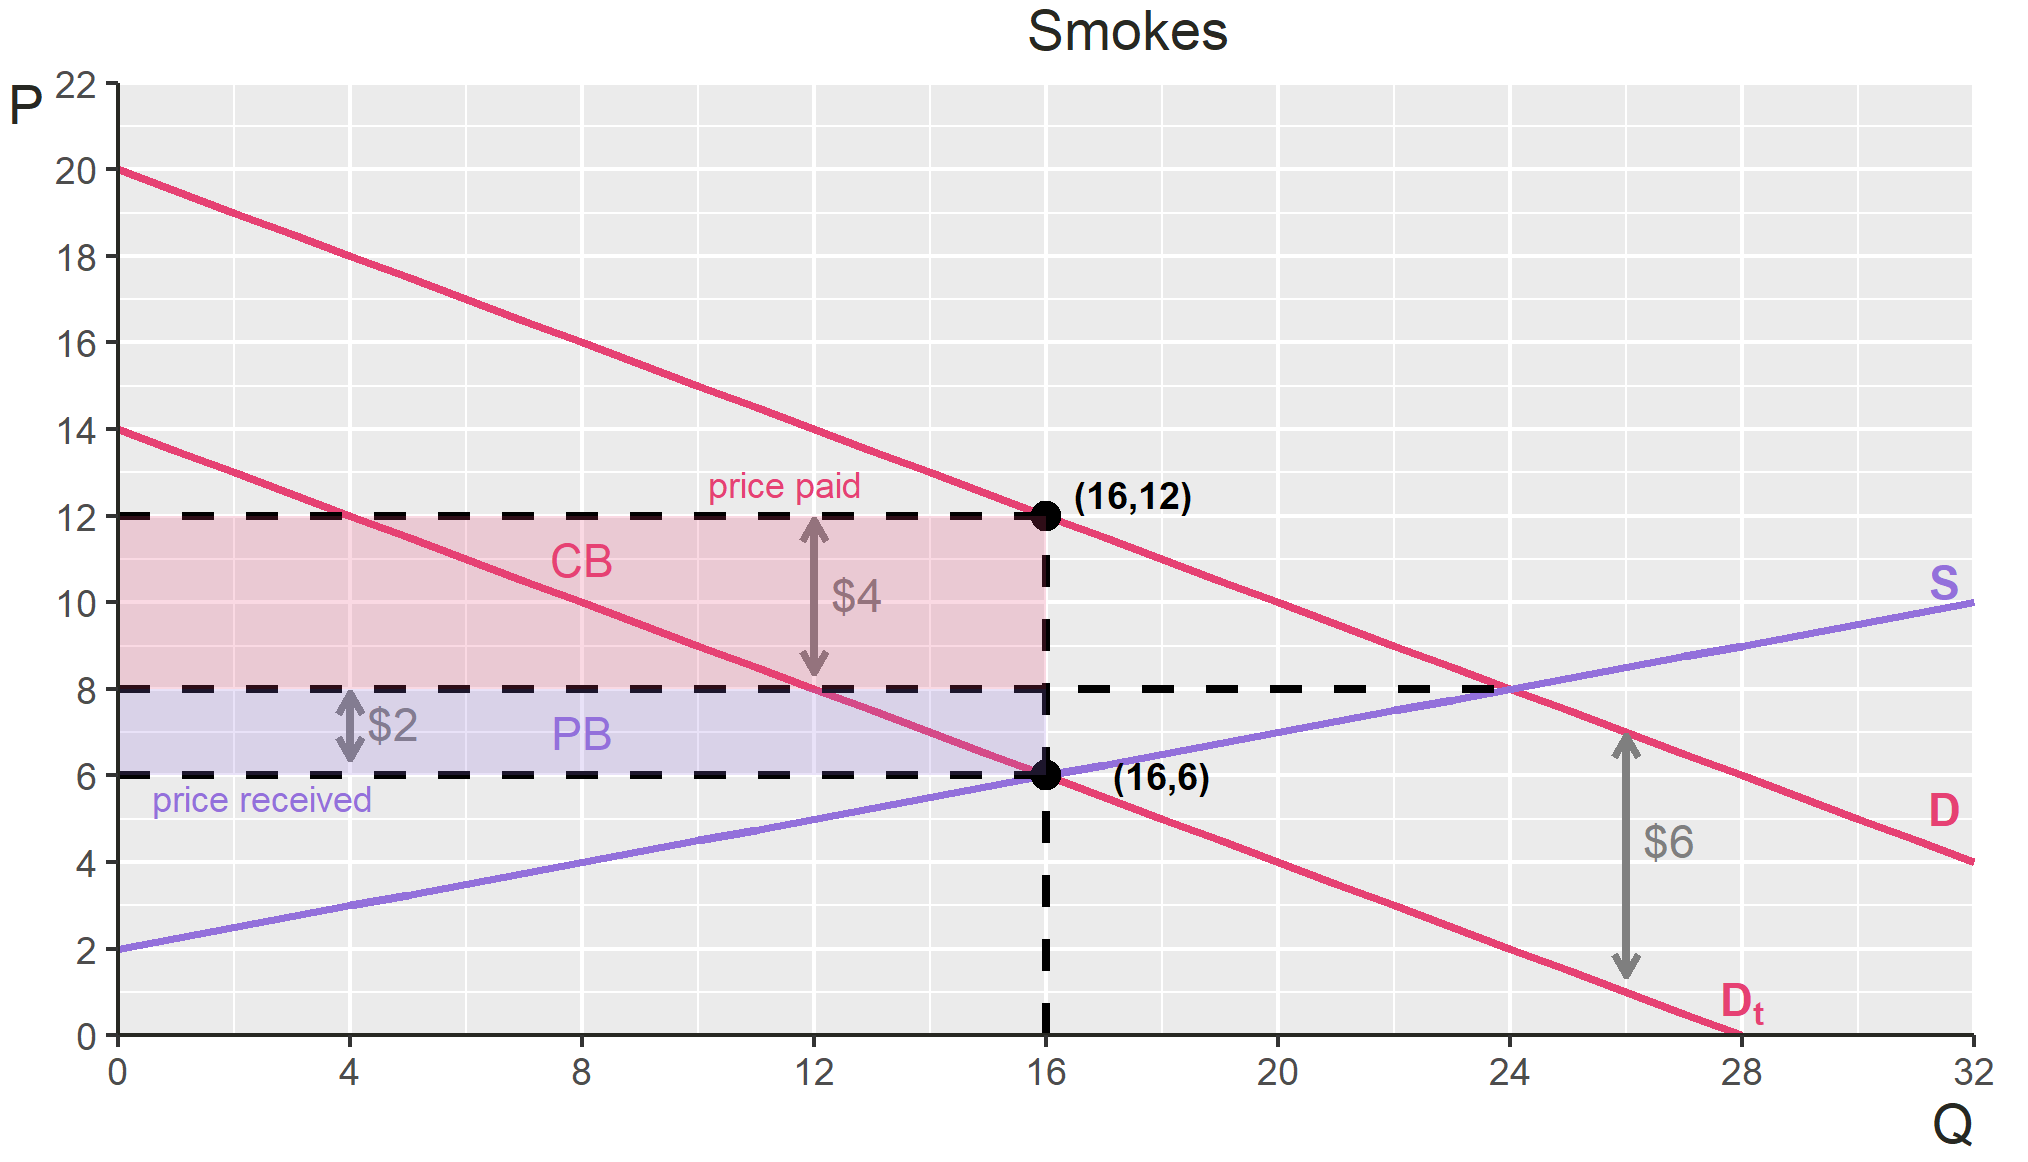
\includegraphics[width=8cm]{Dart tax burdens.png}
        \end{figure}
        \vspace{-4mm}
    \begin{itemize}[<+->]
        \item Consumers bear $\$4$/unit, producers bear $\$2$/unit
        \item Note that these are only in terms of per-unit burdens, the full burden on consumers and producers can be found by calculating the area of the rectangles above
    \end{itemize}
\end{frame}

\begin{frame}{Tax Burden -- Tax on Consumers}
        \begin{figure}
            \centering
            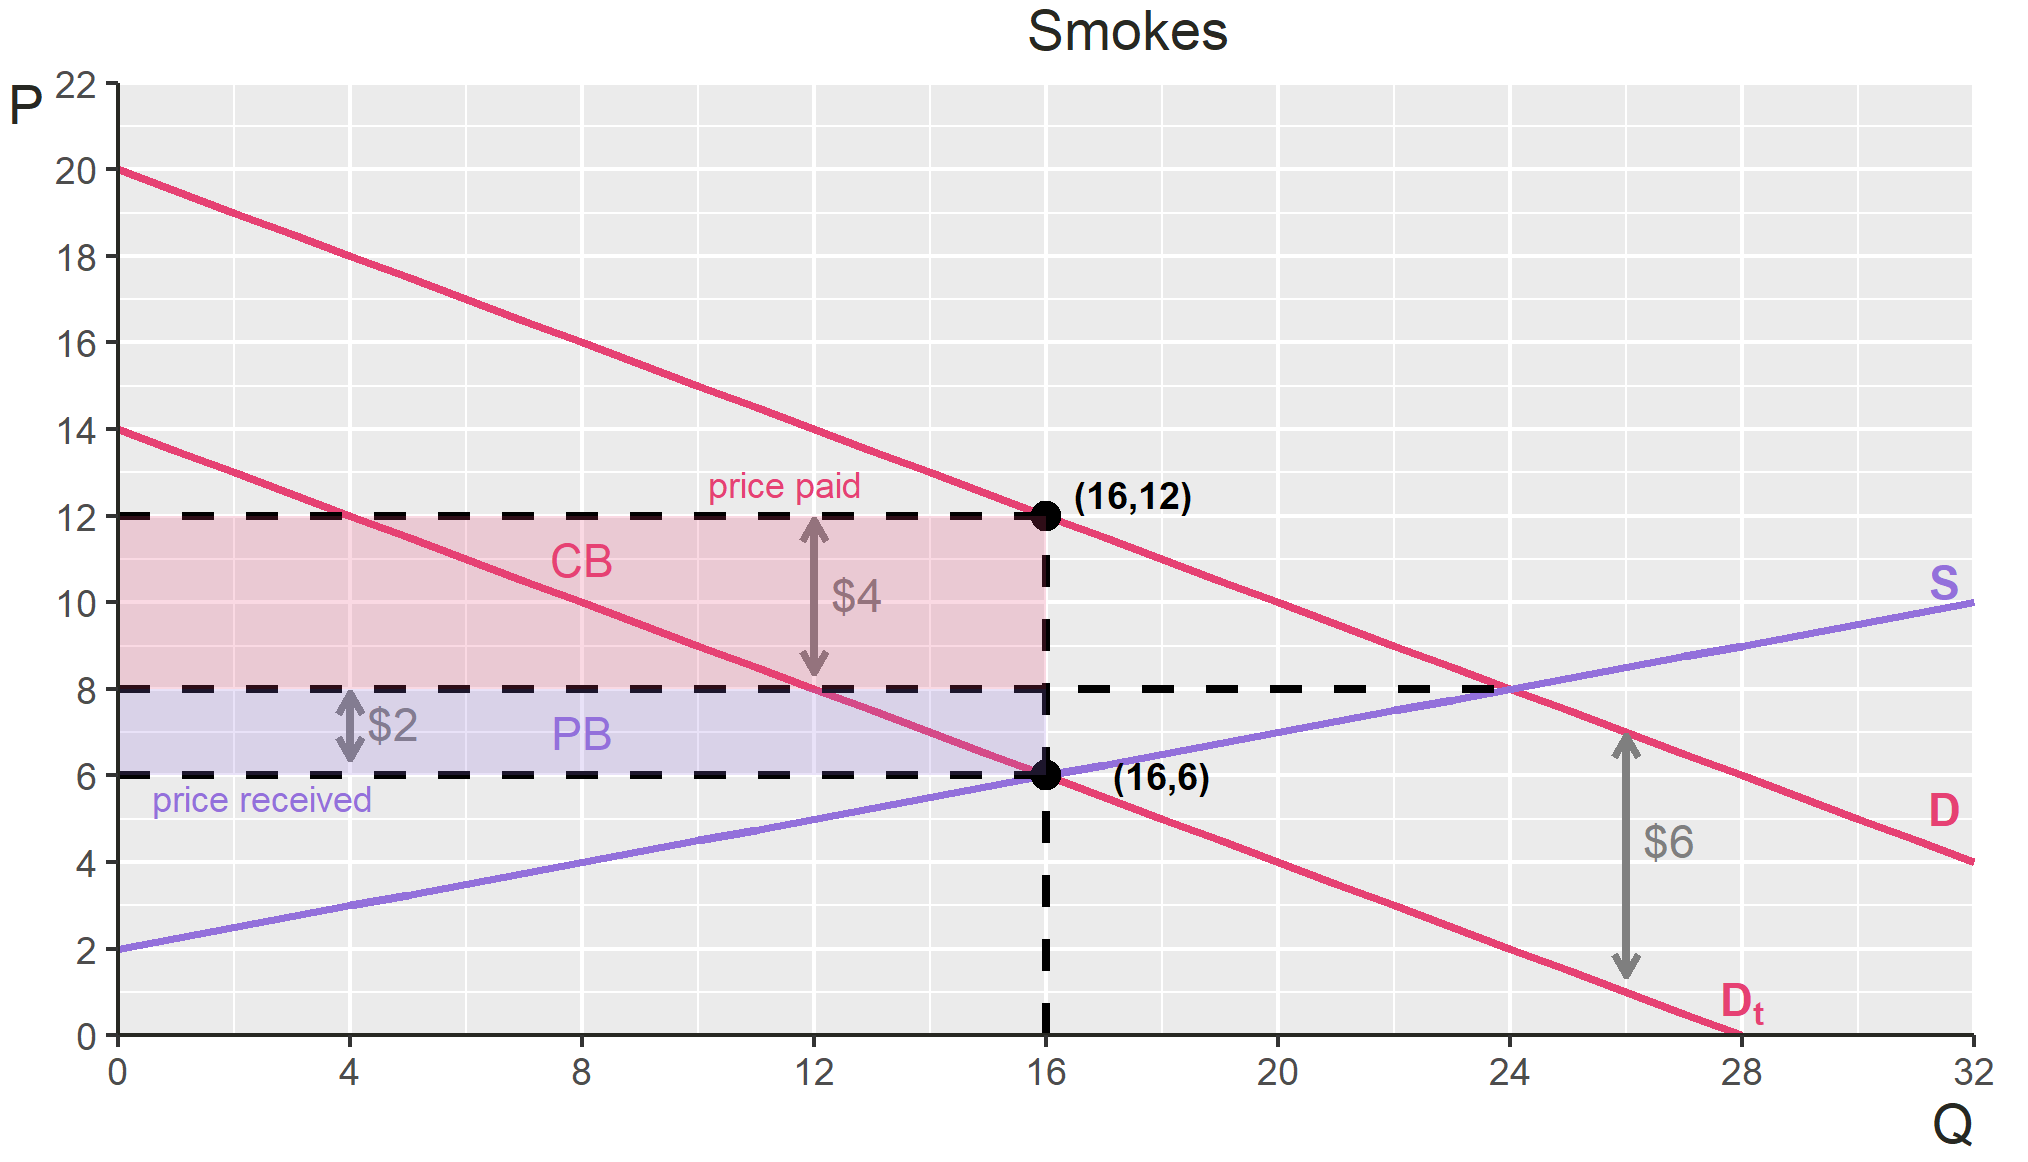
\includegraphics[width=8cm]{Dart tax burdens.png}
        \end{figure}
        \vspace{-4mm}
    \begin{itemize}[<+->]
        \item Namely, the full consumer burden is $(4)(16)=64$, while the full producer burden is $(2)(16)=32$
        \item Also note: The total tax burden is exactly the area of government revenue, which should make sense
    \end{itemize}
\end{frame}

\begin{frame}{Tax Burden -- Tax on Producers}
    \begin{itemize}[<+->]
        \item Recall our oil example:
        \begin{figure}
            \centering
            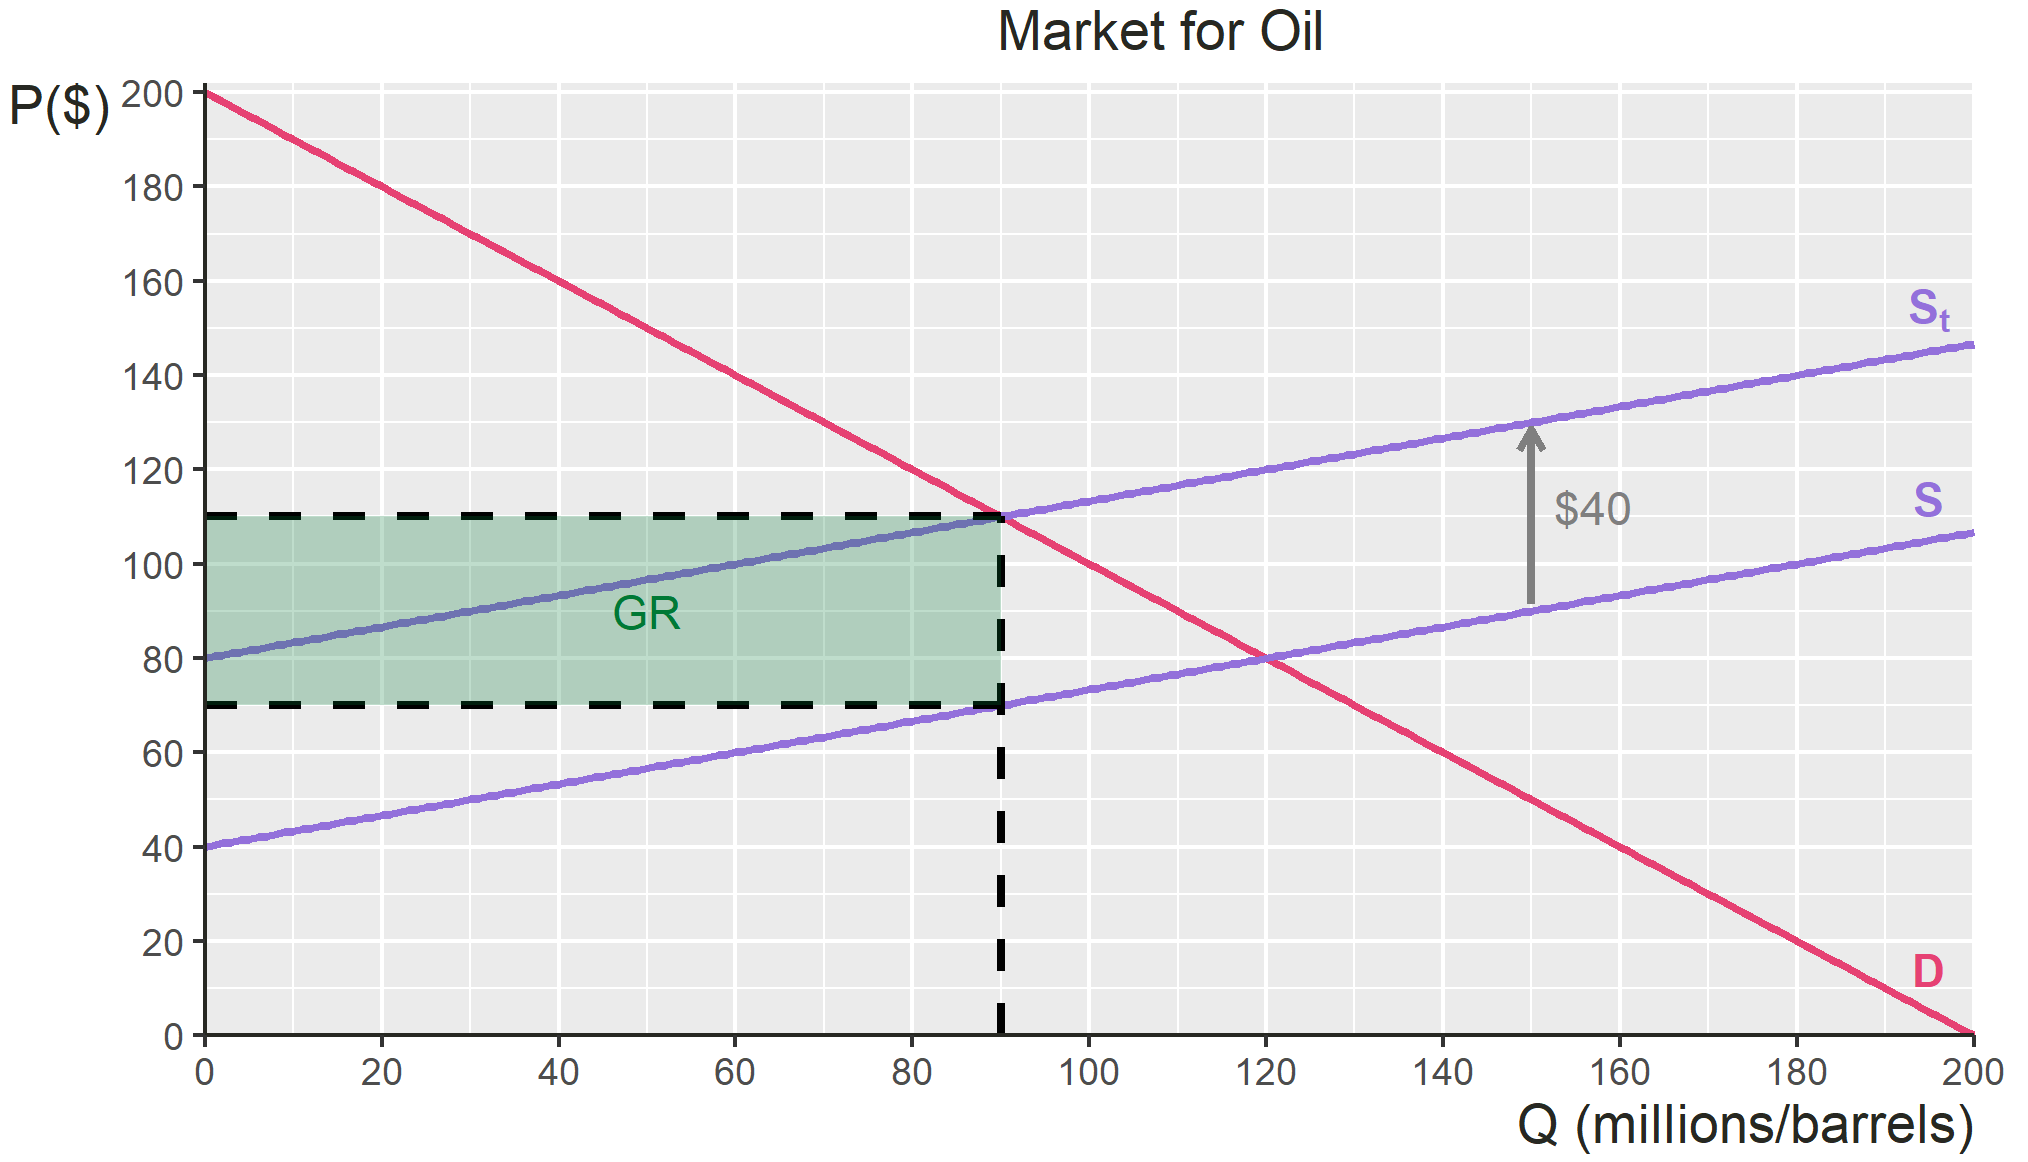
\includegraphics[width=8cm]{Oil tax gr.png}
        \end{figure}
        \item What are the CB and PB in this diagram?
    \end{itemize}
\end{frame}

\begin{frame}{Tax Burden -- Tax on Producers}
    \begin{itemize}[<+->]
        \item Consumers/producers used to pay/receive $\$80$, now the consumers pay $\$110$ and the producers receive $\$70$
        \begin{figure}
            \centering
            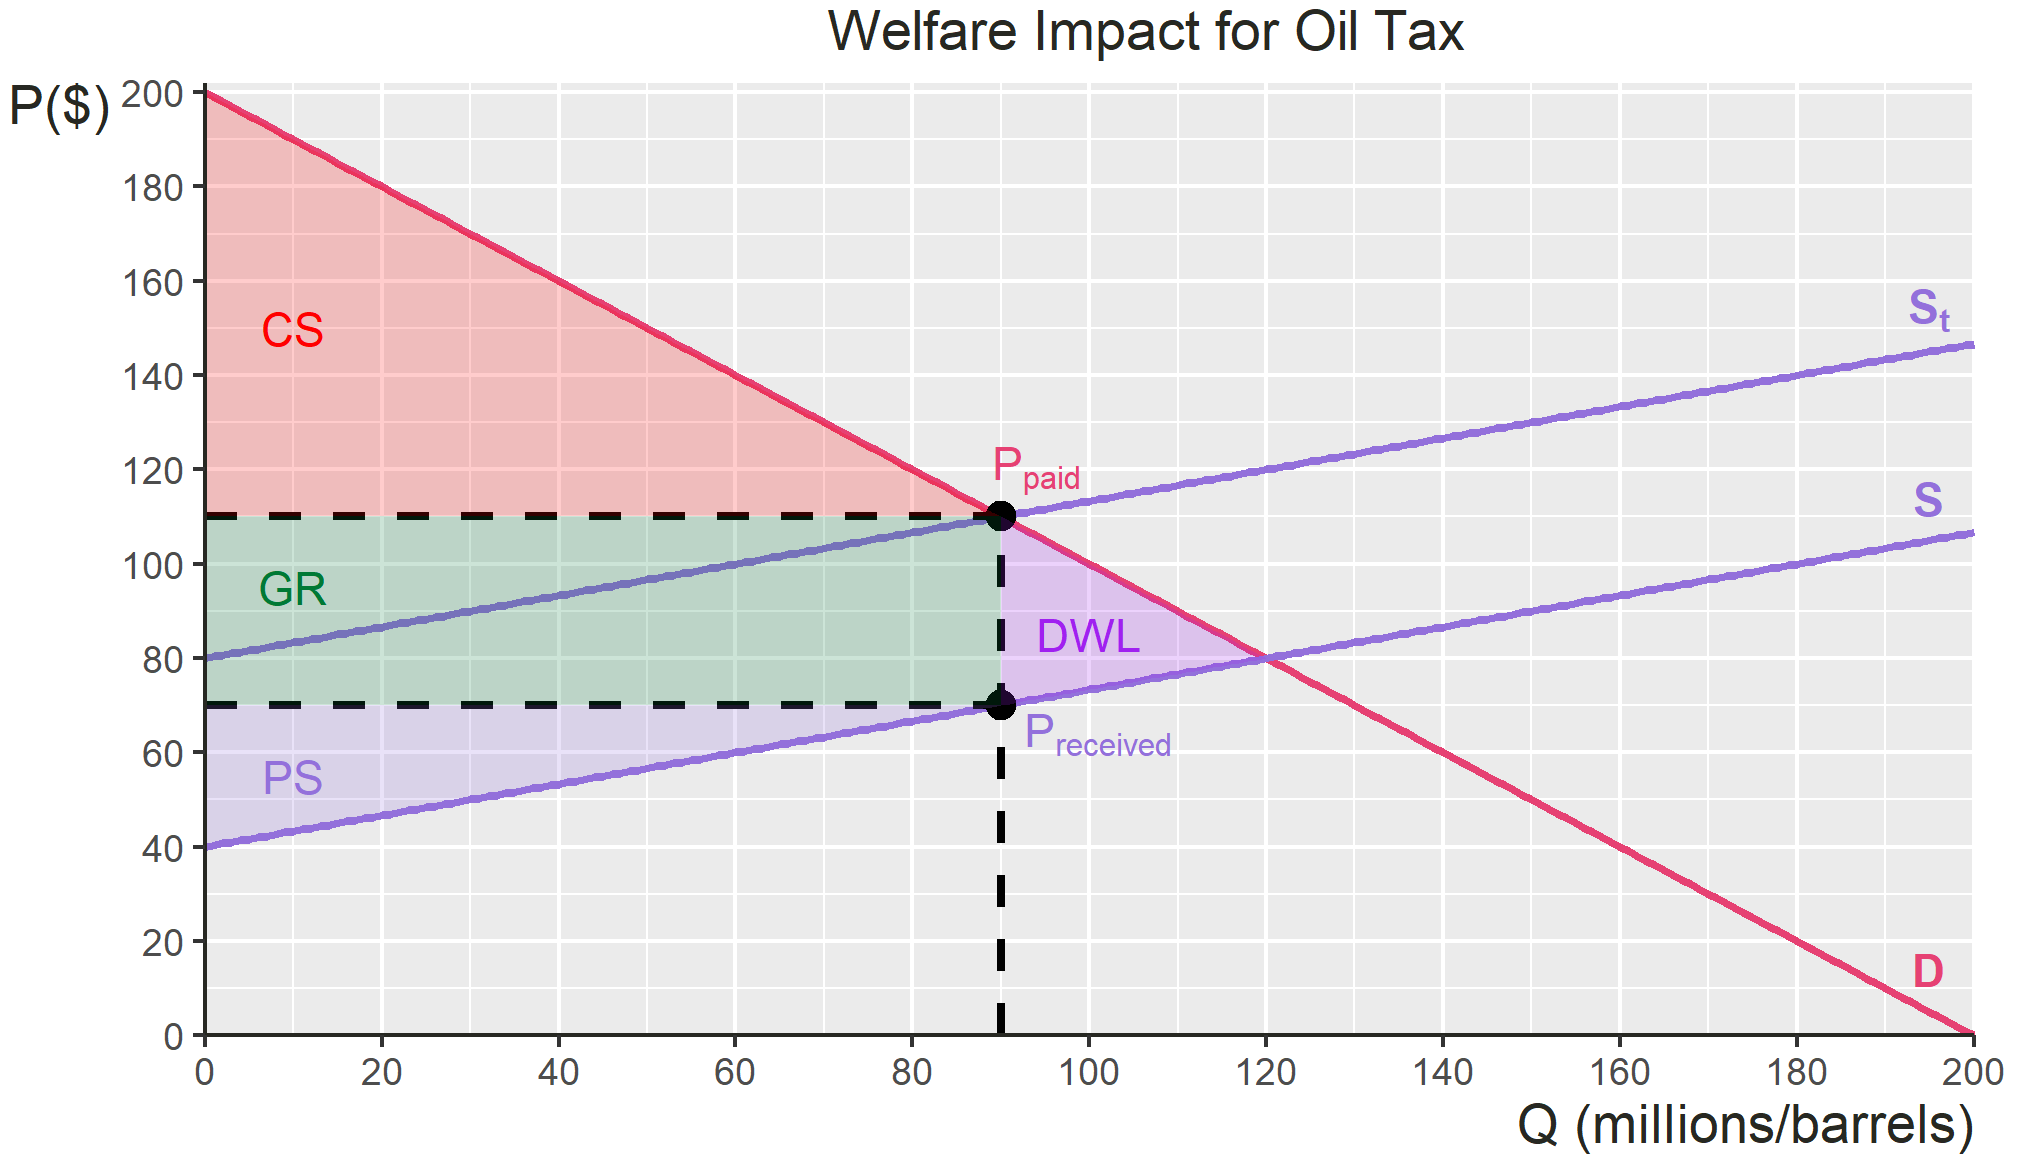
\includegraphics[width=8cm]{Oil tax burdens.png}
        \end{figure}
        \vspace{-2mm}
        \item Therefore, the consumers pay $\$30$/unit of the burden, while consumers pay $\$10$/unit
        \item What are the full burdens?
    \end{itemize}
\end{frame}

\begin{frame}{Subsidy Incidence}
    \begin{itemize}[<+->]
        \item We can do the same thing for a subsidy: while we might physically give a tax return to consumers, the stimulation in demand will just drive prices up, meaning producers effectively take some of that 
        \item The subsidy incidence (or burden) is defined identically to the tax burden
        \begin{itemize}
            \item The subsidy incidence is the difference between what consumers (producers, resp.) \textit{used to} pay (receive), and what they \textit{currently} pay (receive)
        \end{itemize}
        \item Looking at the subsidy incidence very similar to looking at the tax burden
        \begin{itemize}
            \item Again, it just uses the original equilibrium to divide the government expenditure to consumers/producers
            \item However, now it is reversed: Consumer incidence is on the bottom, producers incidence is on the top 
        \end{itemize}
    \end{itemize}
\end{frame}

\begin{frame}{Subsidy Incidence -- Subsidy on Consumers}
    \begin{itemize}[<+->]
        \item Recall our solar panel subsidy from last class:
        \begin{figure}
            \centering
            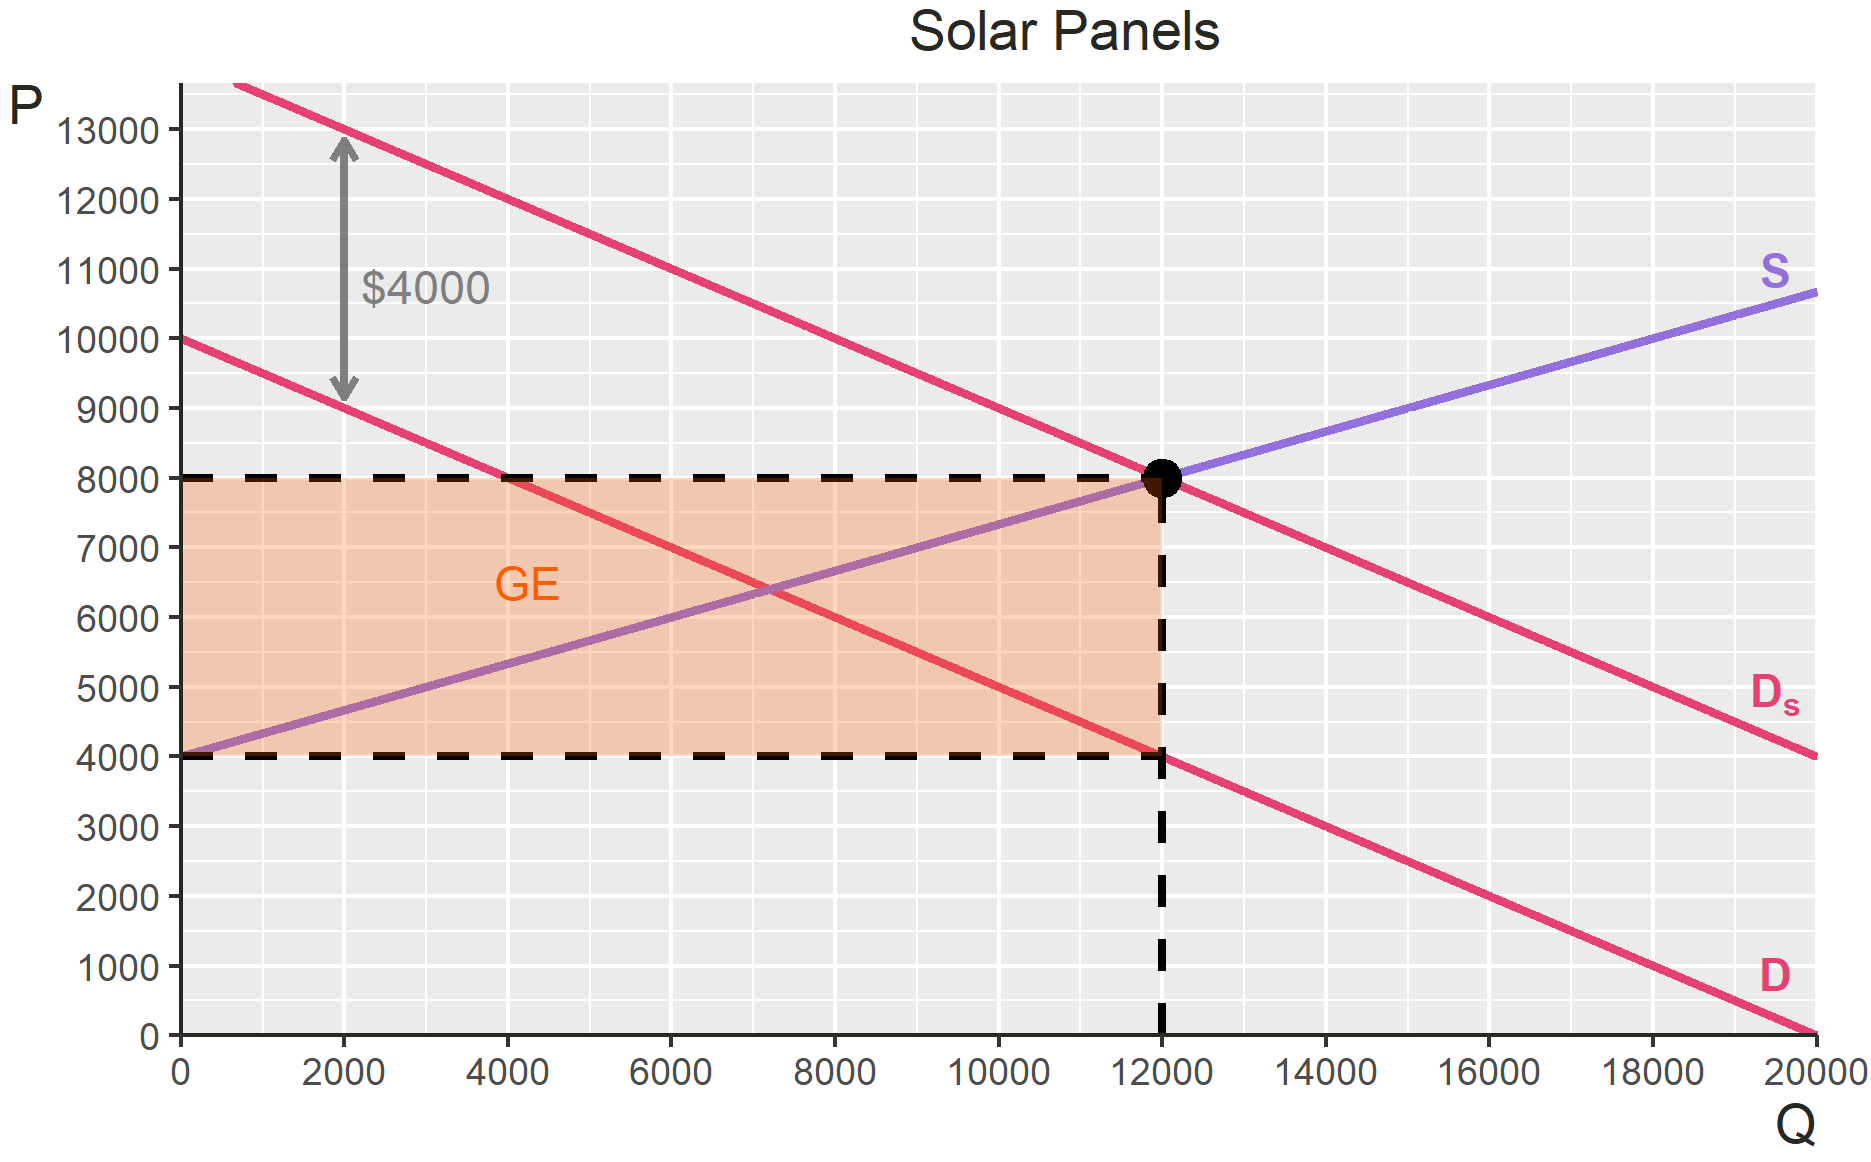
\includegraphics[width=8cm]{Solar sub ge.png}
        \end{figure}
        \item Note: the original equilibrium price is $\$6400$
    \end{itemize}
\end{frame}

\begin{frame}{Subsidy Incidence -- Subsidy on Consumers}
    \begin{itemize}[<+->]
        \item The per-unit producer incidence is $8000-6400=\$1600$, while the per-unit consumer incidence is $6400-4000=\$2400$
        \begin{figure}
            \centering
            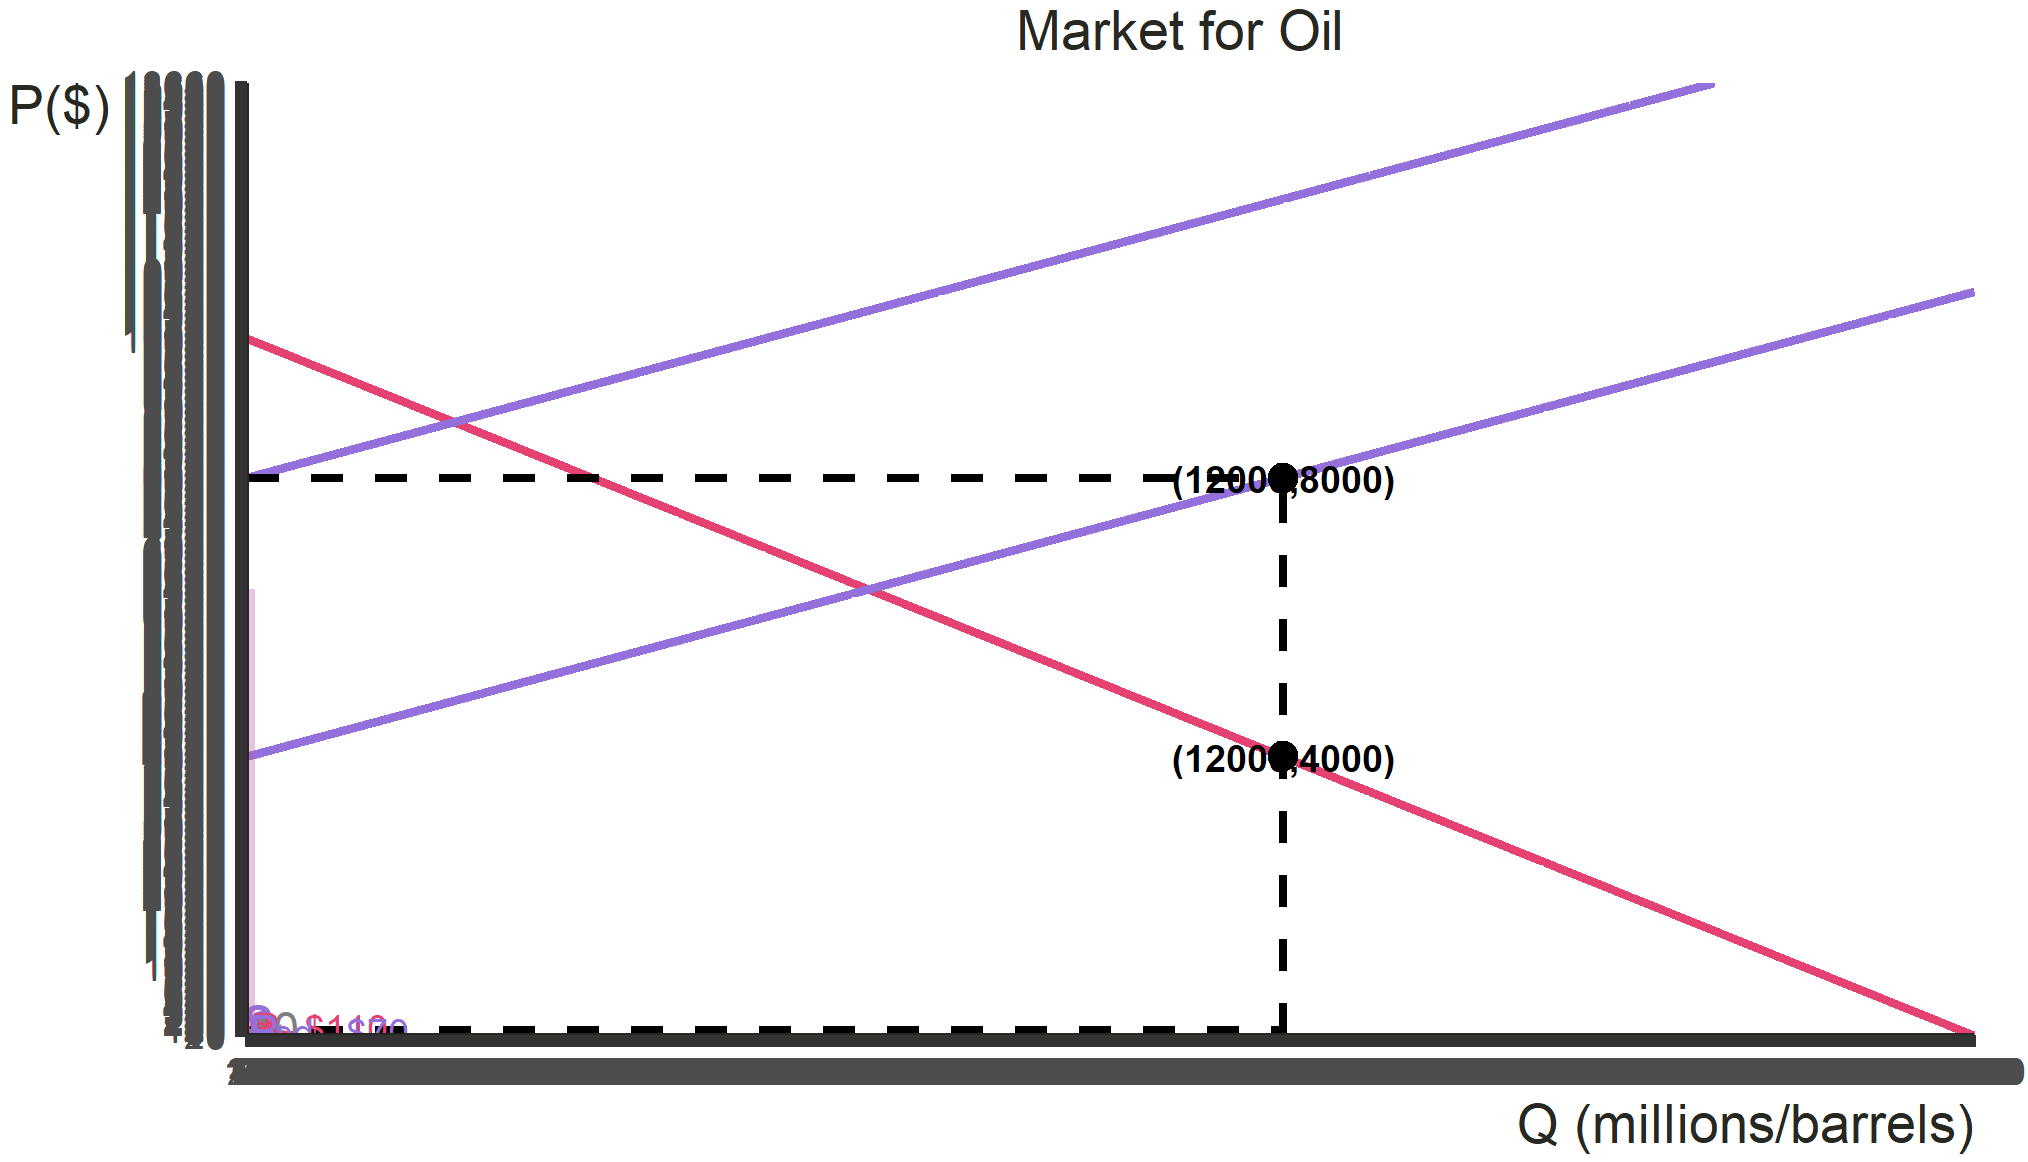
\includegraphics[width=8cm]{Solar sub burdens.png}
        \end{figure}
        \item What are full CI and PI?
    \end{itemize}
\end{frame}

\begin{frame}{Remarks}
    \begin{itemize}[<+->]
        \item Note that when we have a tax -- no matter who it's on -- consumers pay more than producers receive
        \begin{itemize}
            \item Moreover, consumers pay more than they did in the original case, and producers receive less than they originally did
        \end{itemize}
        \item On the other hand, we have a subsidy producers receive more than consumers pay
        \begin{itemize}
            \item Moreover, consumers pay less than they originally did, and producers receive more than they originally did
        \end{itemize}
        \item This is exactly by design of taxes/subsidies
        \item Finally, go back and note that the burden/incidence for each party flips depending on whether we are in a tax or a subsidy, just like prices paid/received do
        \item It is for this reason that studying/understanding these graphs is very important -- it's too much to memorize
    \end{itemize}
\end{frame}

\section*{Taxes and Welfare}

\begin{frame}{Redefining Total Surplus}
    \begin{itemize}[<+->]
        \item To talk about welfare with taxes and subsidies, we must update our definition of total surplus in the economy:
        \begin{itemize}
            \item Total surplus is \textit{increased} by government revenue
            \item Total surplus is \textit{decreased} by government expenditure
        \end{itemize}
        \item While we may never include a tax and a subsidy on the same diagram, the formula becomes
        $$TS=CS+PS+GR-GE$$
        \item Motivation: you can think of the government as a party that can now have positive or negative surplus
        \begin{itemize}
            \item In reality, our motivation is that with tax revenue, the government can spend money on public goods and services, improving the economy
            \item Conversely, when it spends money, it no longer has the funds to do those things\footnote{The funds it is spending, on subsidies in this case, are being counted as TS good through the CS or PS route}
        \end{itemize}
    \end{itemize}
\end{frame}

\begin{frame}{How to Think about CS Under a Consumption Tax}
    \begin{itemize}[<+->]
        \item Recall that consumer surplus is...
        \begin{itemize}
            \item The difference between what consumers were willing to pay and what they actually paid
        \end{itemize}
        \item Recall that before, the demand curve is a reflection of willingness to pay
        \item Now, under a consumption tax, the original demand line \textit{is still the proper reflection of willingness to pay}
        \item In some sense, the taxed demand line $D_{t}$ is more about determining equilibrium quantity and the price that the producer receives -- the consumer is still willing to pay according to the demand $D$
    \end{itemize}
\end{frame}

\begin{frame}{How to Think about CS Under a Tax}
\begin{figure}
    \centering
    \includegraphics[width=7cm]{Dart tax cs.png}
\end{figure}
    \begin{itemize}[<+->]
        \item In the figure above, CS is area from the price that consumers pay, to the WTP (original demand) curve
        \item Even though the consumers pay 
    \end{itemize}
\end{frame}

\begin{frame}{How to Think about CS Under a Tax}
\begin{figure}
    \centering
    \includegraphics[width=7cm]{Dart tax cs.png}
\end{figure}
    \begin{itemize}[<+->]
        \item Remark: If you want to abandon the way I teach this, you can technically count CS as the area from price received ``equilibrium price" to the new demand line
        \begin{itemize}
            \item Not only does your figure get uglier, as you will see in a minute, but this muddles the interpretation of consumer surplus
        \end{itemize}
    \end{itemize}
\end{frame}

\begin{frame}{Total Surplus -- A Tax on Consumers}
    \begin{itemize}[<+->]
        \item The other areas carry the same definition as before, creating this nice diagram:
        \begin{figure}
            \centering
            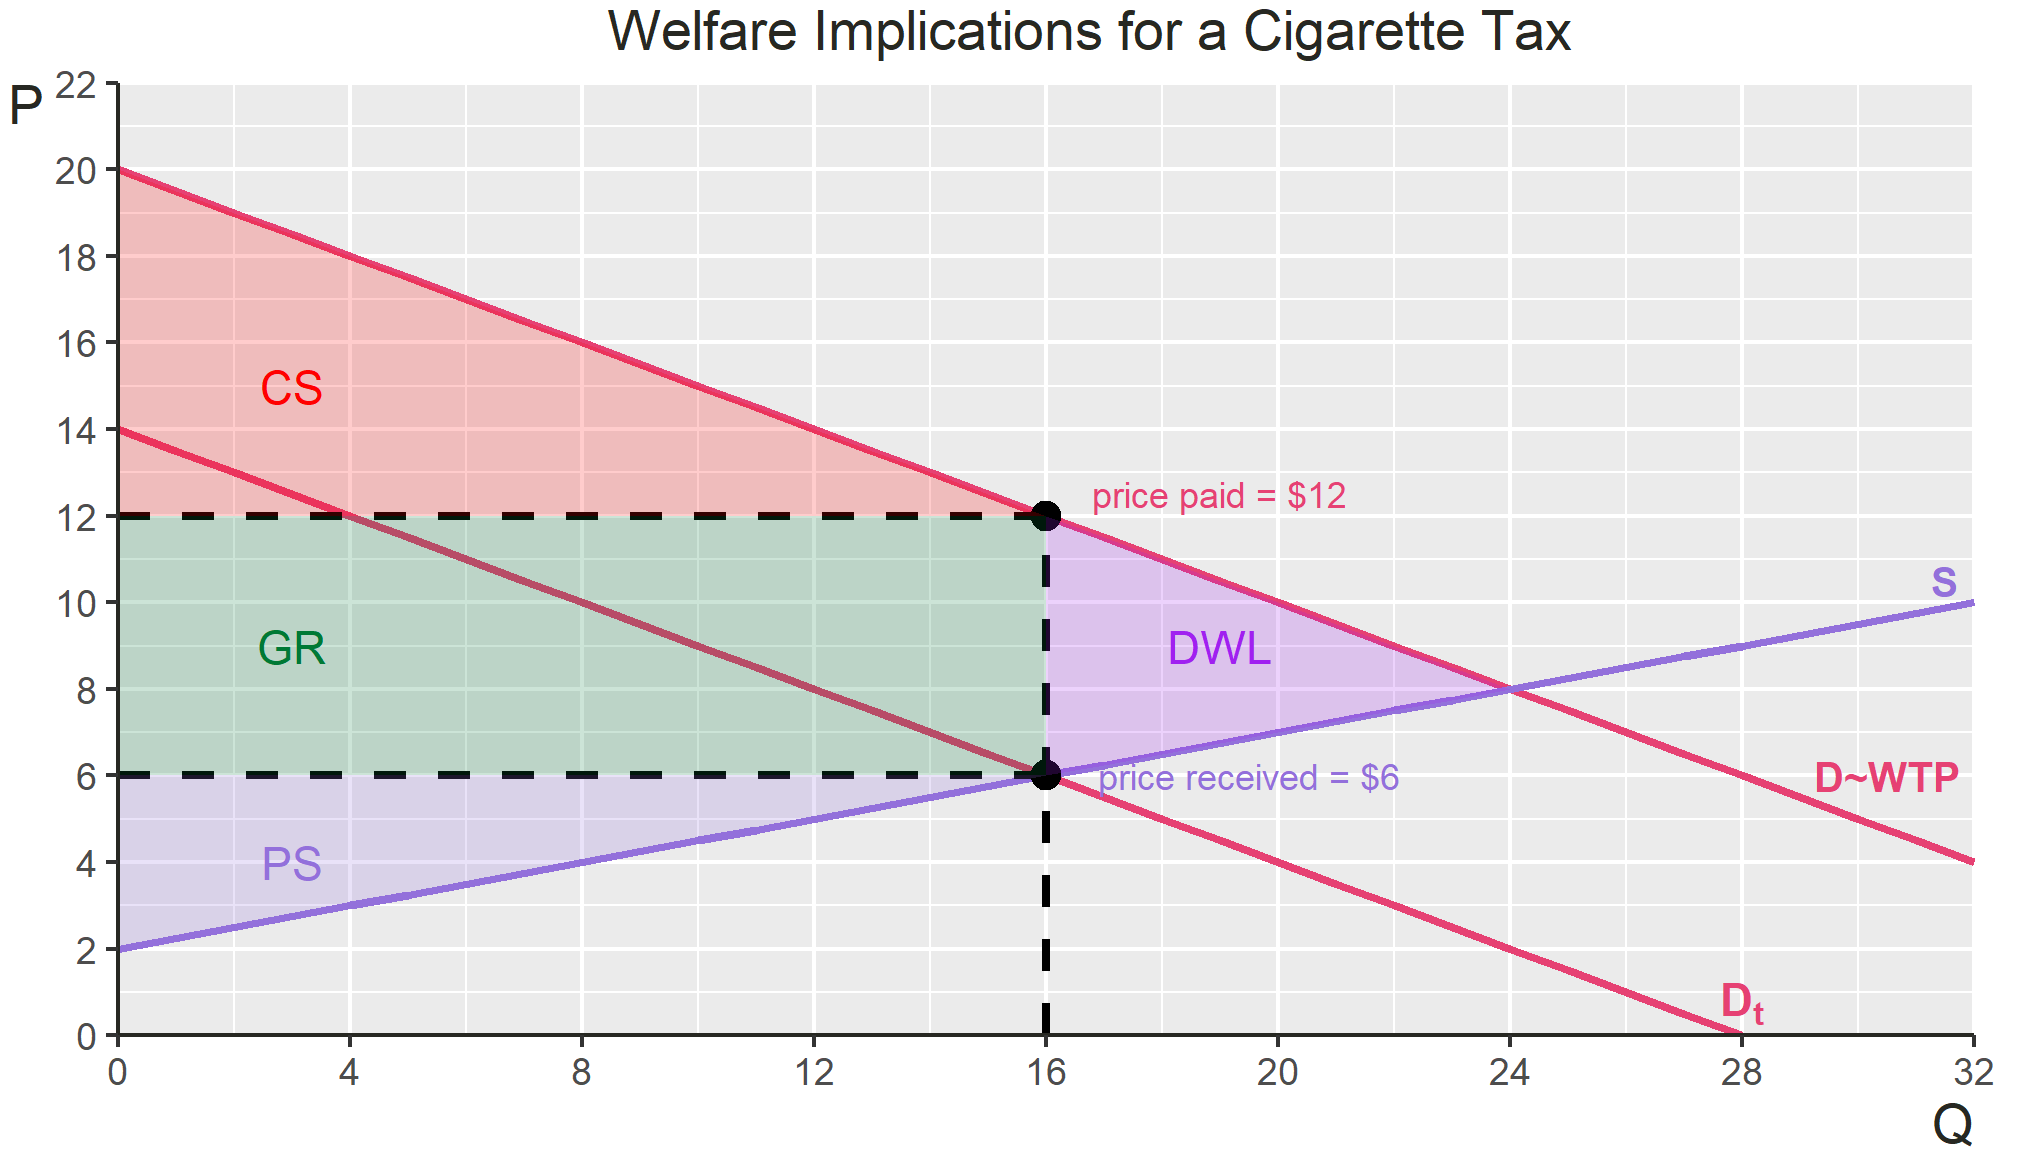
\includegraphics[width=9cm]{Dart tax ts.png}
        \end{figure}
    \end{itemize}
\end{frame}

\begin{frame}{Total Surplus -- A Tax for Producer}
    \begin{itemize}[<+->]
        \item The same is true for PS under a production tax: the supply curve is still the proper reflection for willingness to pay
        \item Thus, the TS diagram looks like:
        \begin{figure}
            \centering
            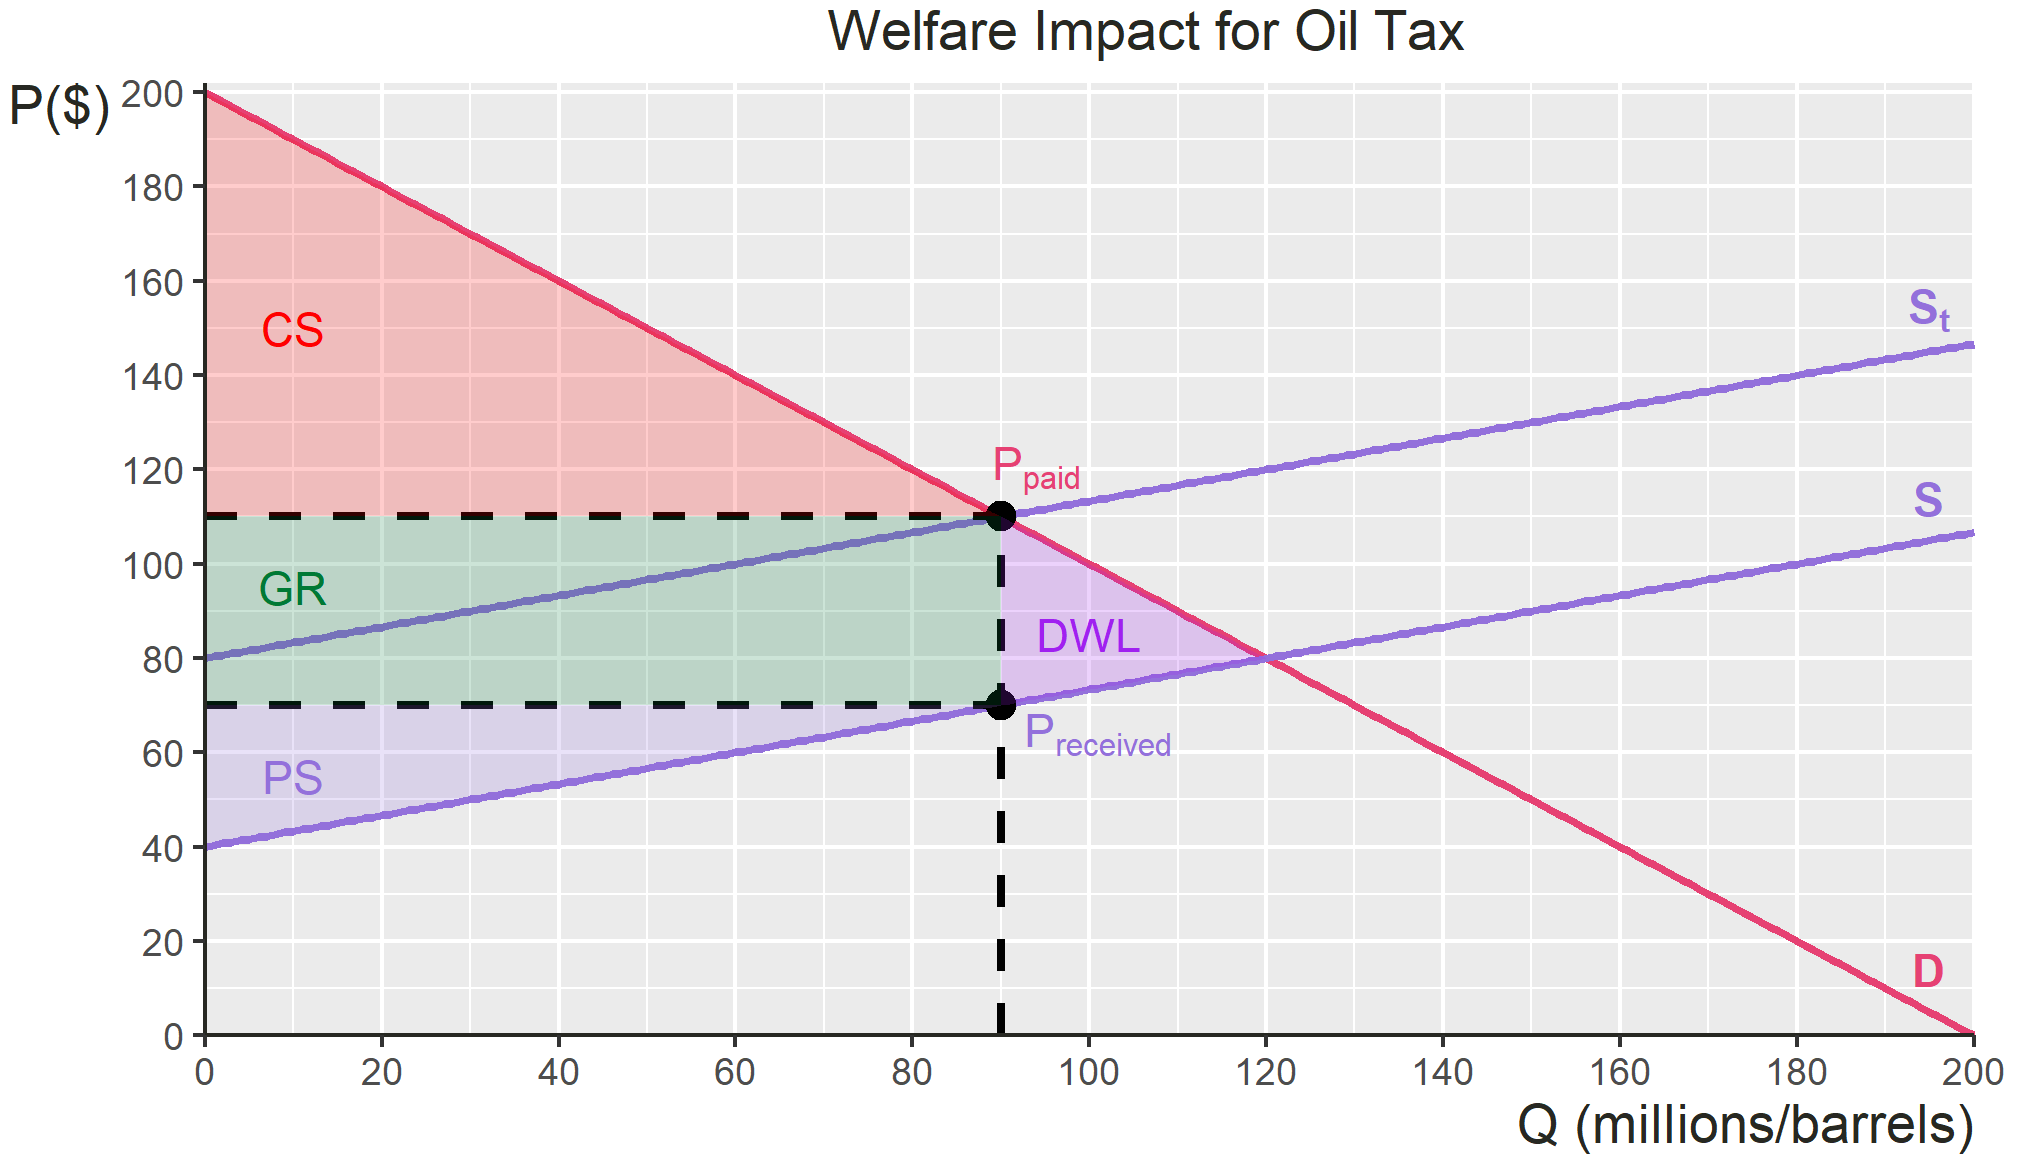
\includegraphics[width=9cm]{Oil tax welfare.png}
        \end{figure}
    \end{itemize}
\end{frame}

\begin{frame}{How to Think about CS/PS Under a Subsidy}
    \begin{itemize}[<+->]
        \item All of the intuition for thinking about Subsidies is the same as for taxes, but the picture isn't quite as pretty
        \item Again, there are technically multiple ways to draw the right area 
        \item I will teach you the one that is consistent with our definitions
        \item Here are the general rules:
        \begin{itemize}
            \item CS is the difference between WTP and price paid, PS is the difference between price received and WTA 
            \item Original demand represents WTP, original supply represents WTA
            \item Always remember that DWL is the difference between optimal TS and new TS
        \end{itemize}
    \end{itemize}
\end{frame}

\begin{frame}{Total Surplus -- A Subsidy for Consumers}
    \begin{itemize}[<+->]
        \item Recall this example:
        \begin{figure}
            \centering
            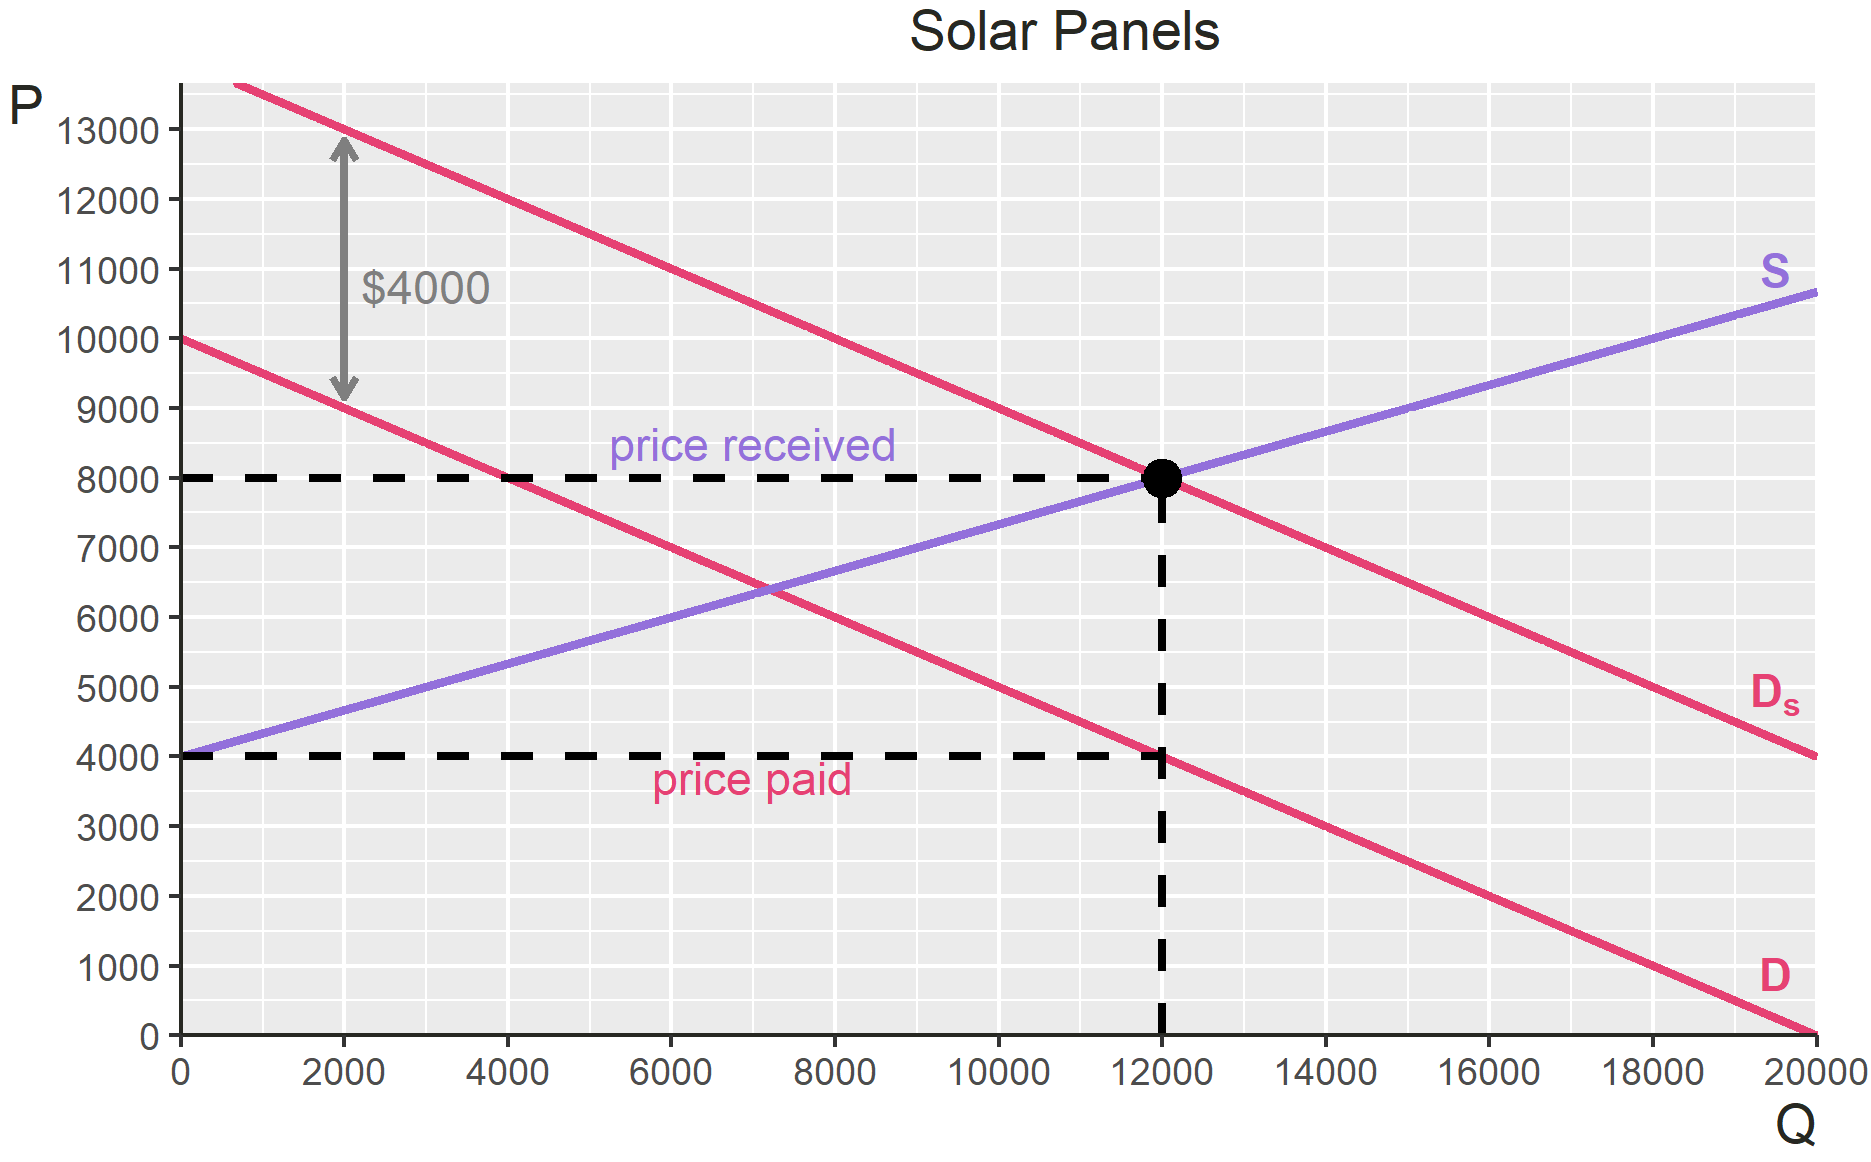
\includegraphics[width=8cm]{Solar sub prices.png}
        \end{figure}
    \end{itemize}
\end{frame}

\begin{frame}{CS -- A Subsidy for Consumers}
    \begin{itemize}[<+->]
        \item CS is shown below
        \begin{figure}
            \centering
            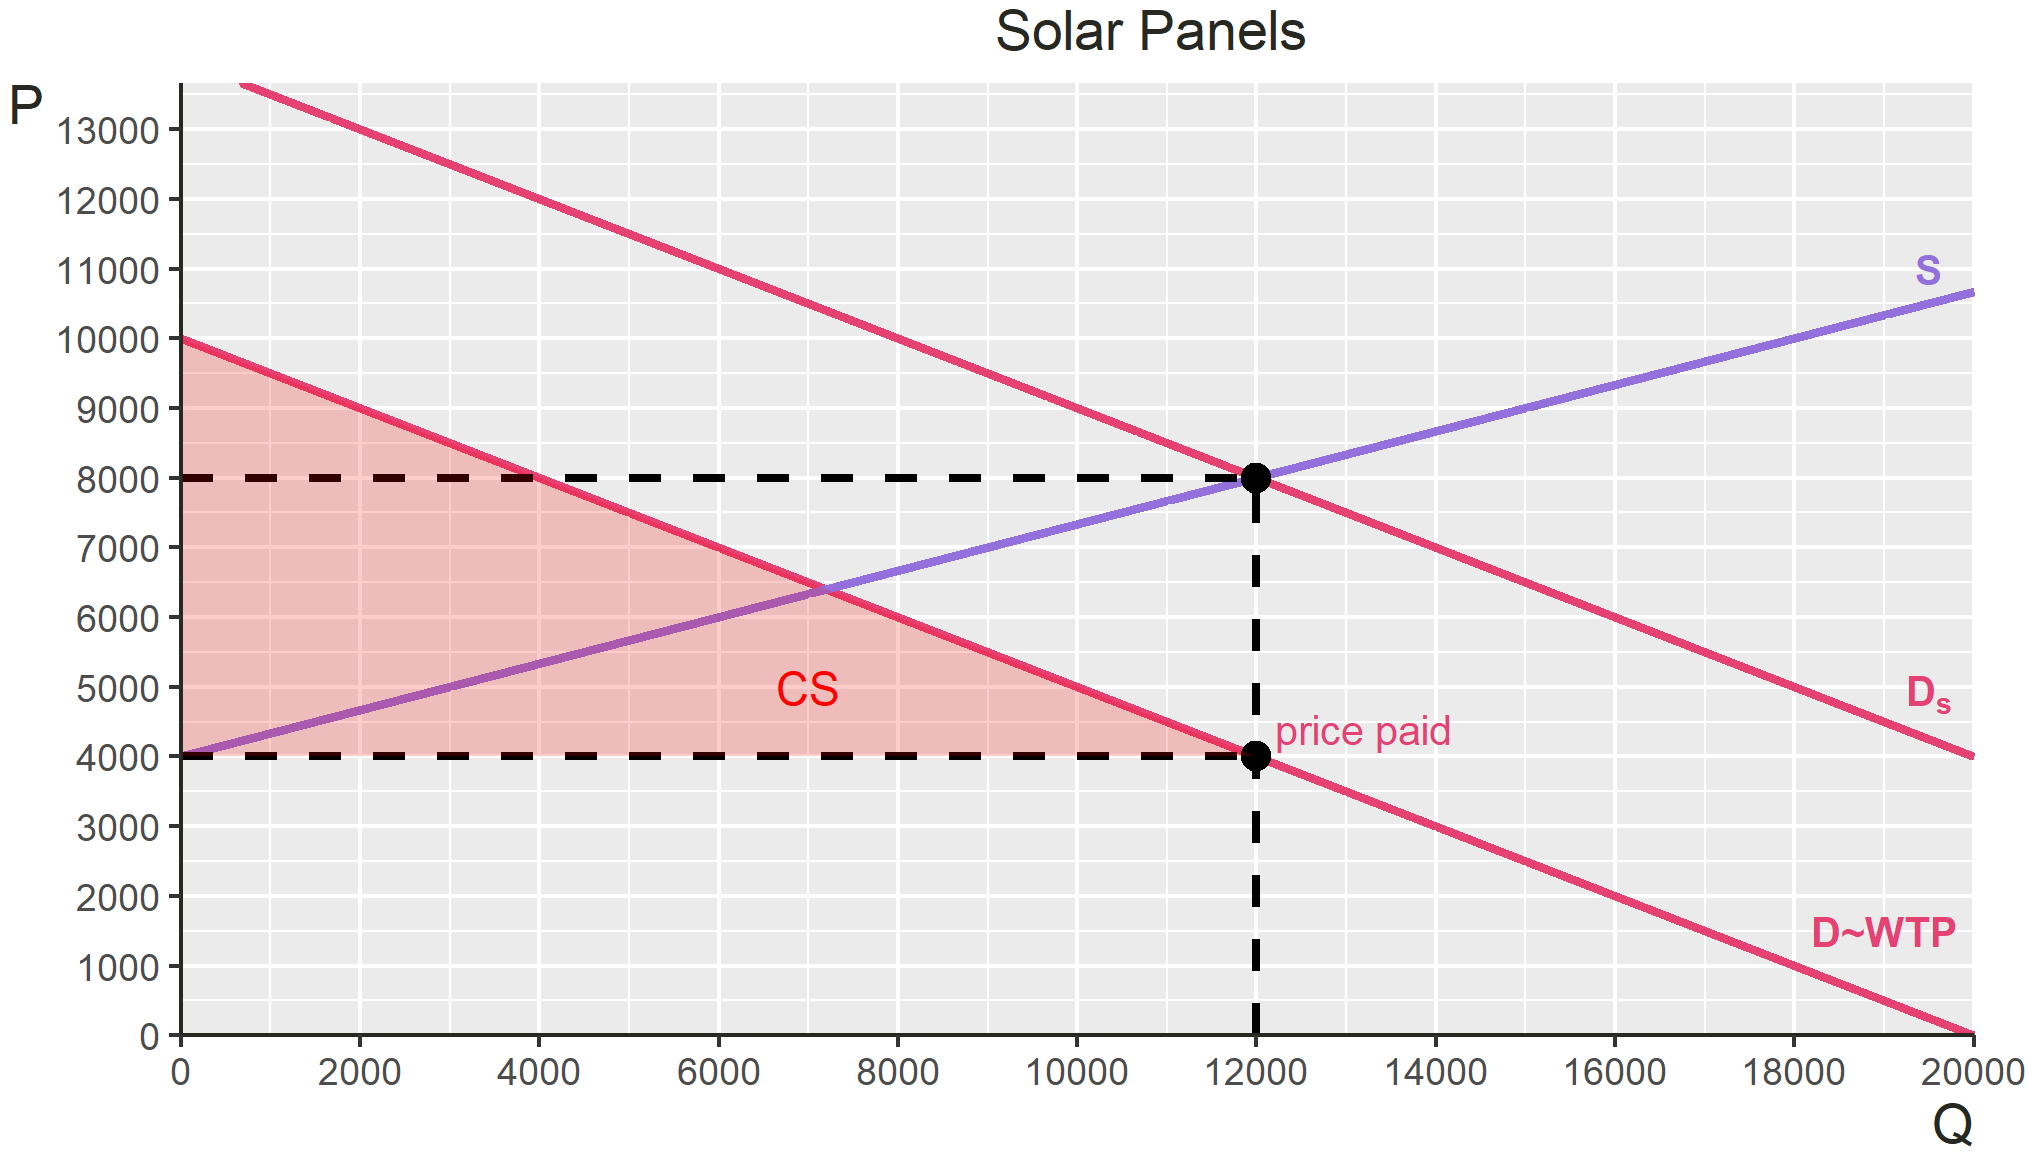
\includegraphics[width=8cm]{Solar sub CS.png}
        \end{figure}
    \end{itemize}
\end{frame}

\begin{frame}{PS -- A Subsidy for Consumers}
    \begin{itemize}[<+->]
        \item PS is shown below
        \begin{figure}
            \centering
            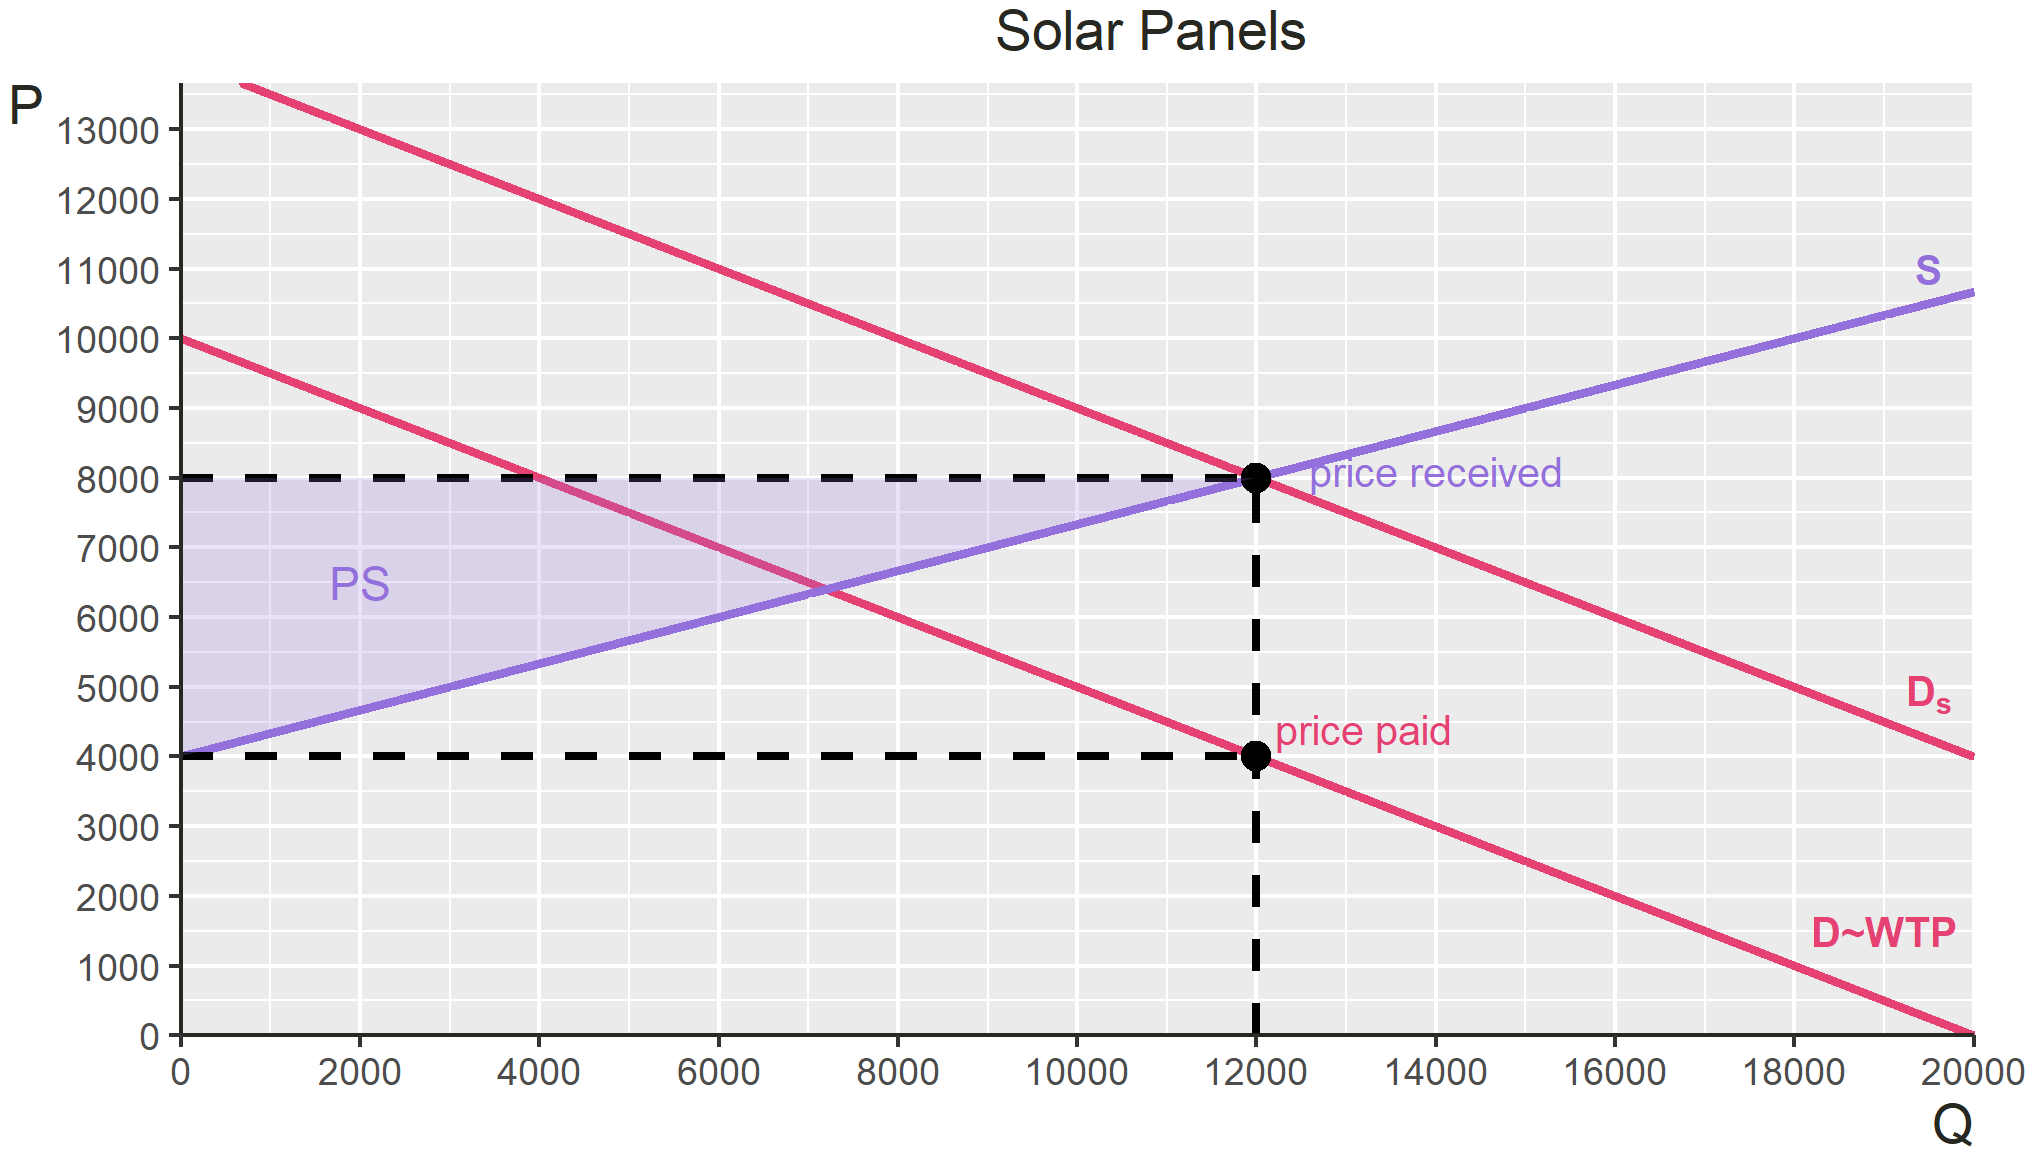
\includegraphics[width=8cm]{Solar sub PS.png}
        \end{figure}
    \end{itemize}
\end{frame}

\begin{frame}{GE -- A Subsidy for Consumers}
    \begin{itemize}[<+->]
        \item GE, which you have already seen, is shown below
        \begin{figure}
            \centering
            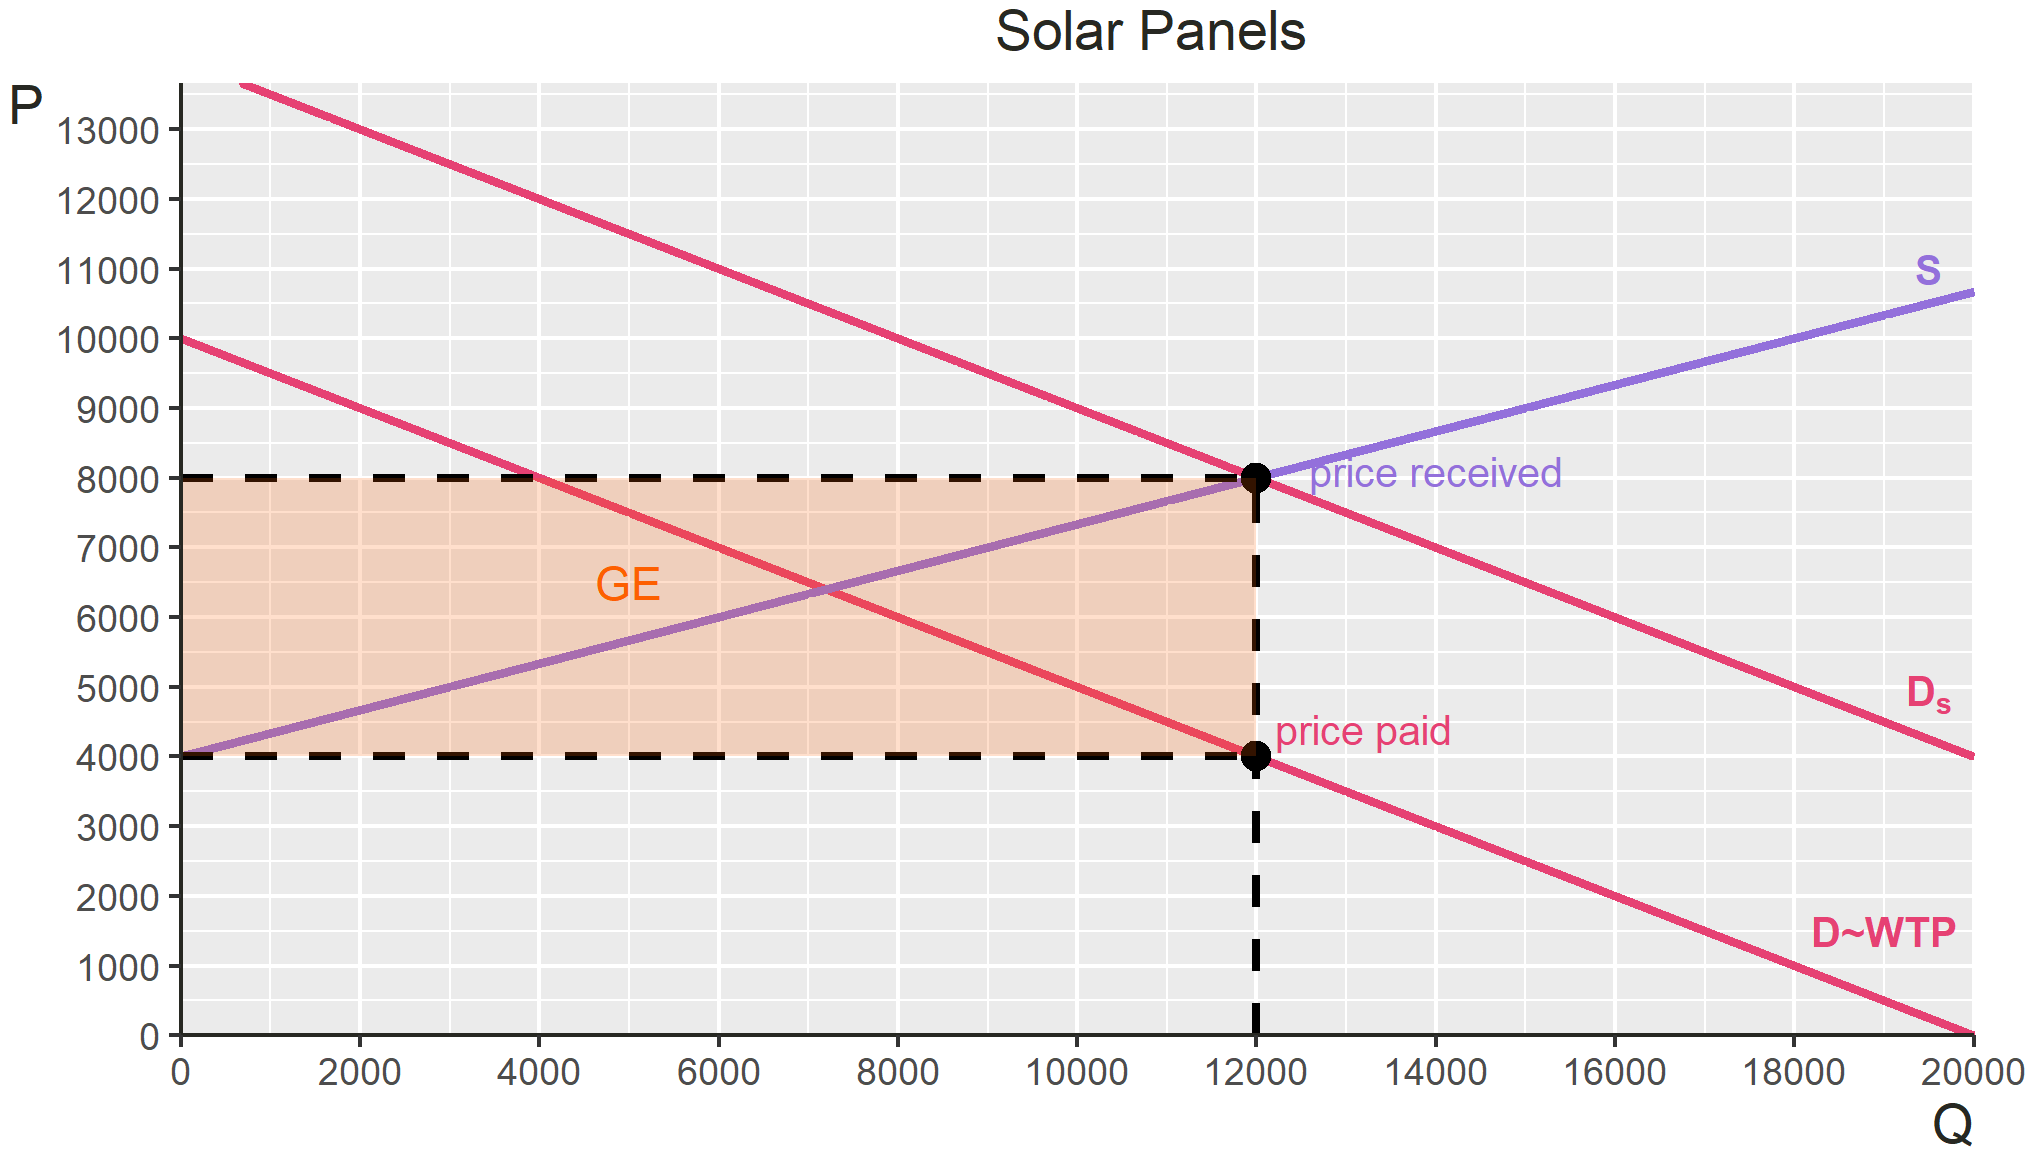
\includegraphics[width=8cm]{Solar sub GE2.png}
        \end{figure}
    \end{itemize}
\end{frame}

\begin{frame}{GE -- A Subsidy for Consumers}
    \begin{itemize}[<+->]
        \item DWL is shown below
        \begin{figure}
            \centering
            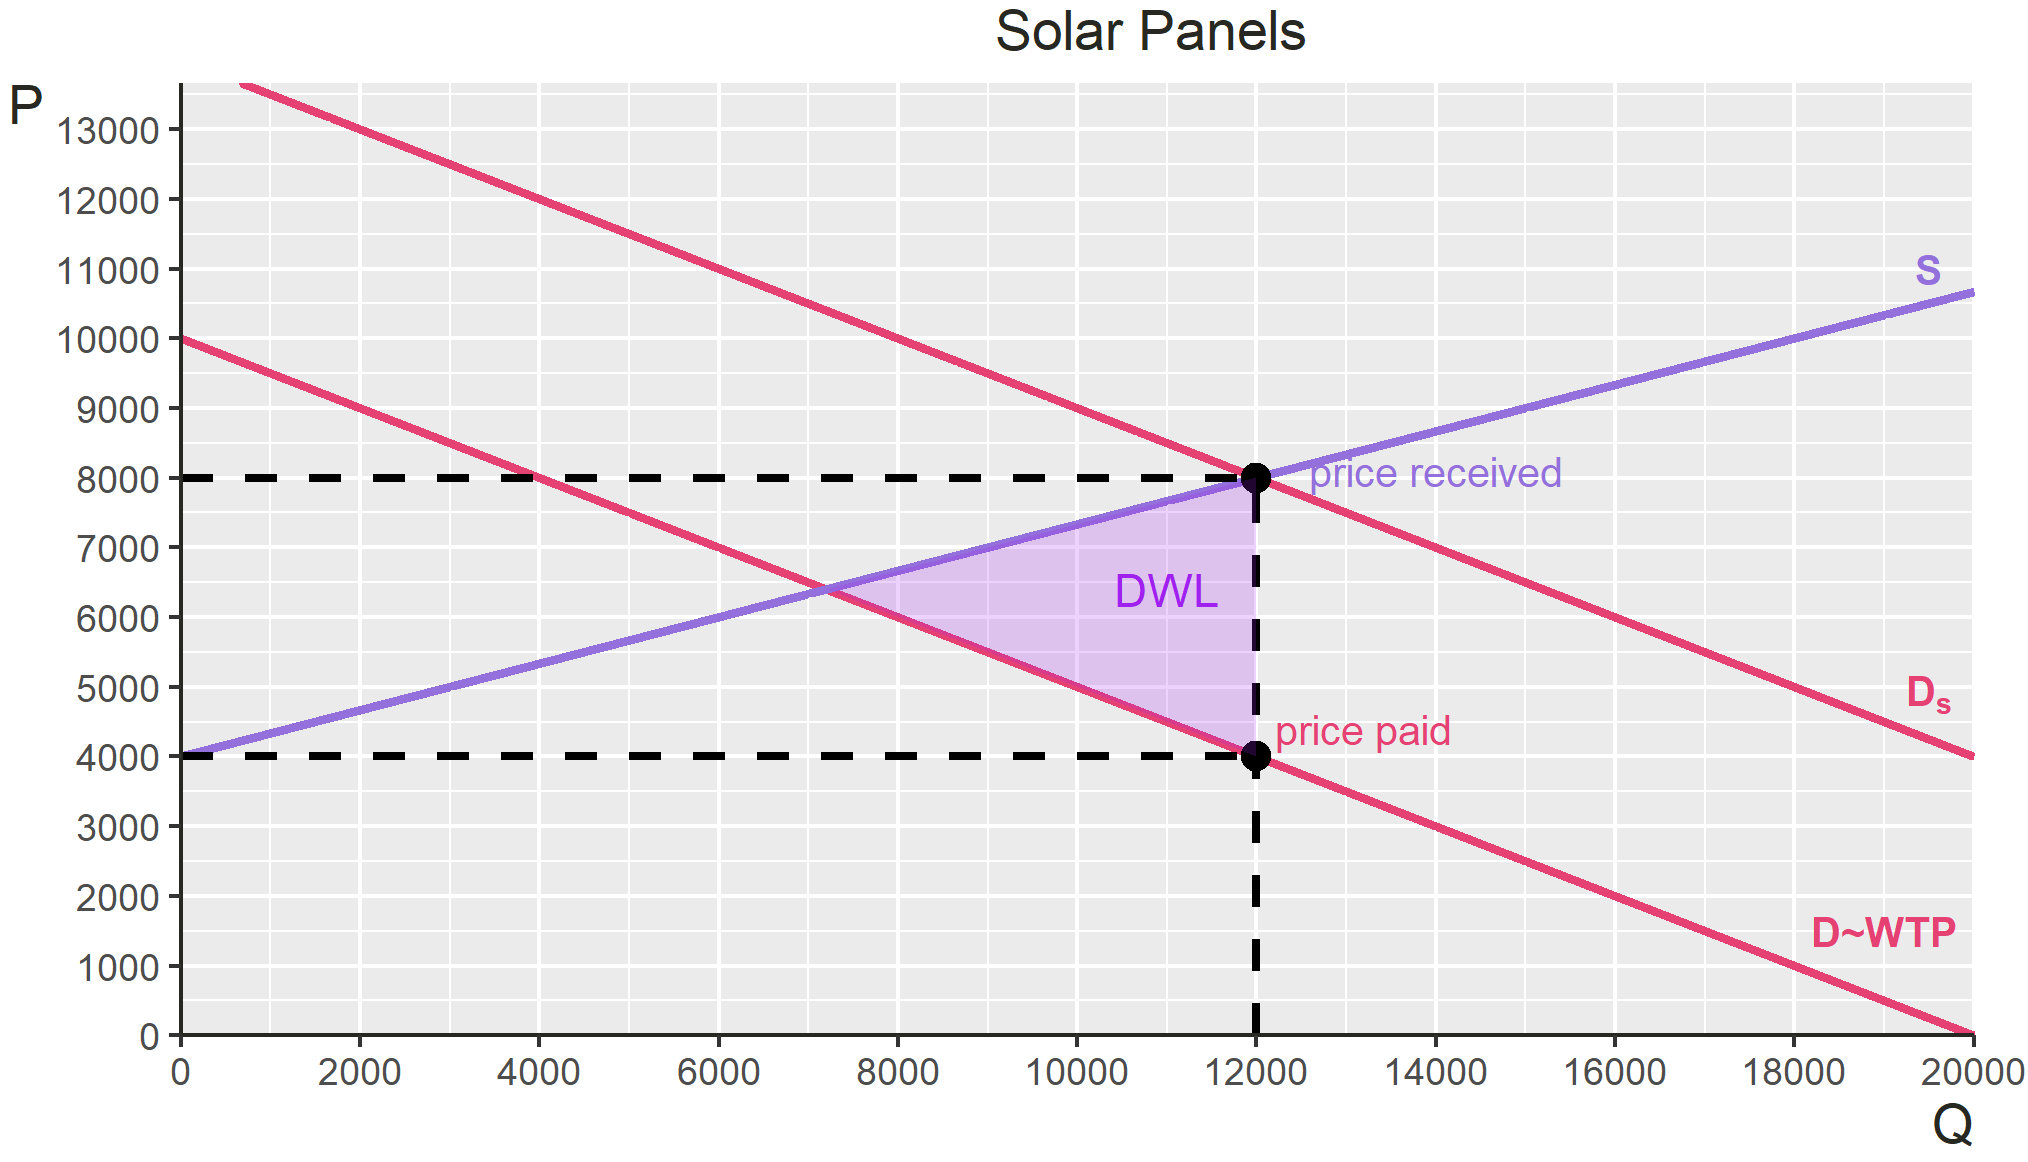
\includegraphics[width=8cm]{Solar sub dwl.png}
        \end{figure}
    \end{itemize}
\end{frame}

\begin{frame}{TS -- A Subsidy for Consumers}
    \begin{itemize}[<+->]
        \item It's fairly challenging to combine everything on on one graph, even with colors
        \item Here is a pretty okay diagram, with consumer/producer burdens, that I drew one time:
        \begin{figure}
            \centering
            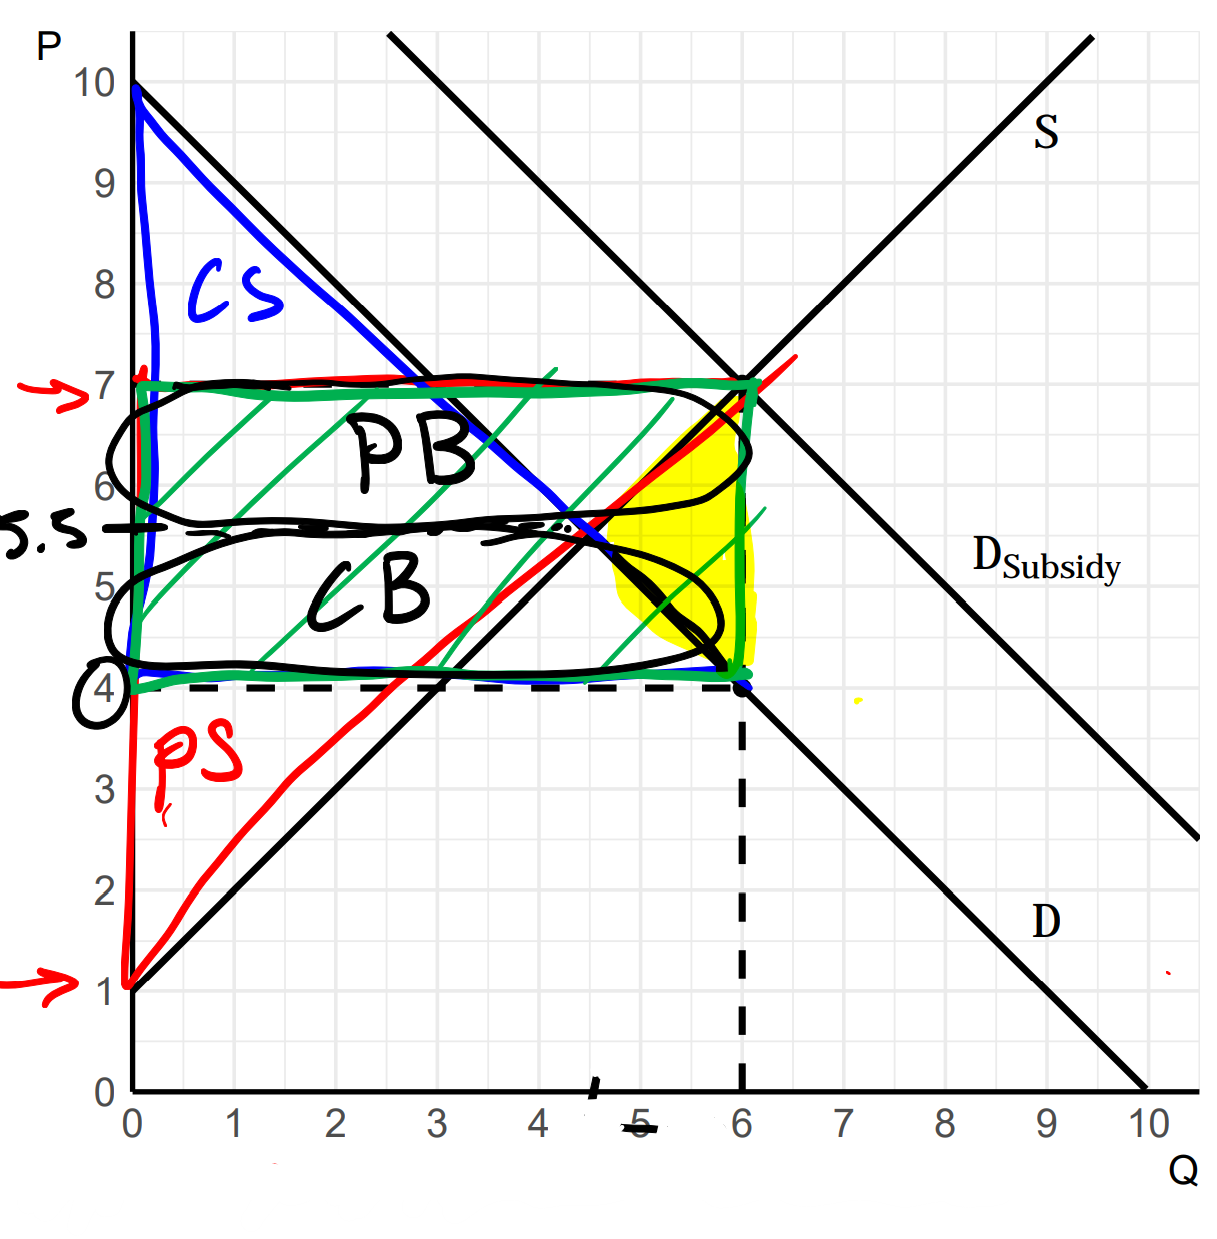
\includegraphics[width=5cm]{Okay drawing of TS.png}
        \end{figure}
    \end{itemize}
\end{frame}

\begin{frame}{Next Time}
    \begin{itemize}[<+->]
        \item I leave the subsidy for producers as an exercise, which you will see in discussion section
        \item Wednesday: Externalities
    \end{itemize}
\end{frame}


\end{document}